\documentclass[preprint,12pt,authoryear] {elsarticle}
%\documentclass[review]{elsarticle}

\usepackage[colorlinks]{hyperref}
\usepackage{lineno}

\modulolinenumbers[5]

%\journal{Ocean Engineering}

\usepackage{amssymb}
\usepackage{amsmath}


\usepackage{subfigure}

\usepackage{epstopdf}
\usepackage{epsfig}
\usepackage{setspace}

\usepackage{ulem}

\newcommand{\be}{\begin{equation}}
\newcommand{\ee}{\end{equation}}
\newcommand{\beq}{\begin{eqnarray}}
\newcommand{\eeq}{\end{eqnarray}}
\newcommand{\ba}{\begin{eqnarray}}
\newcommand{\ea}{\end{eqnarray}}


%%%add
%\documentclass{article}
%\usepackage{natbib}
%\usepackage{cite}
\usepackage{soul}
\doublespacing
\usepackage{color}

%\renewcommand{\tablename}{Table}
\newcommand{\tabincell}[2]{\begin{tabular}{@{}#1@{}}#2\end{tabular}}

\newcommand{\ua}{{\bf u}_\alpha}
\newcommand{\utwo}{\overline{\bf u}_2}



\begin{document}


\begin{frontmatter}

\title{NEARCOM and FUNWAVE-TVD
}


%\author[first]{xxx}

%\address[first]{xxx}

%\begin{abstract}


%\end{abstract}


%\begin{keyword}

%\end{keyword}

\end{frontmatter}

%\linenumbers

\section*{8.6 Hydrodynamic and Wave Modeling (NEARCOM)}

The Nearshore Community Model (NearCoM) is an extensible, user-configurable model system for nearshore wave, circulation and sediment processes developed during the National Oceanographic Partnership Program (NOPP). The model consists of a “backbone”; the master program, handling data input and output as well as internal storage, together with a suite of modules, each of which handles a focused subset of the physical processes being studied (Figure 7,8). A total of 10 modules exists, developed by a large group of researchers from various institutions. Example modules are: 1) A wave module simulates wave transformation over arbitrary coastal bathymetry and predicts radiation stresses and wave-induced mass fluxes; 2) A circulation module simulates the slowly varying current field driven by waves, wind and buoyancy forcing, and provides information on the bottom boundary layer structure; and 3) A seabed module simulates sediment transport, determines the bedform geometry, parameterizes the bedform effect on bottom friction, and computes morphological evolution resulting from spatial variations in local sediment transport rates.

\begin{figure}
\centering
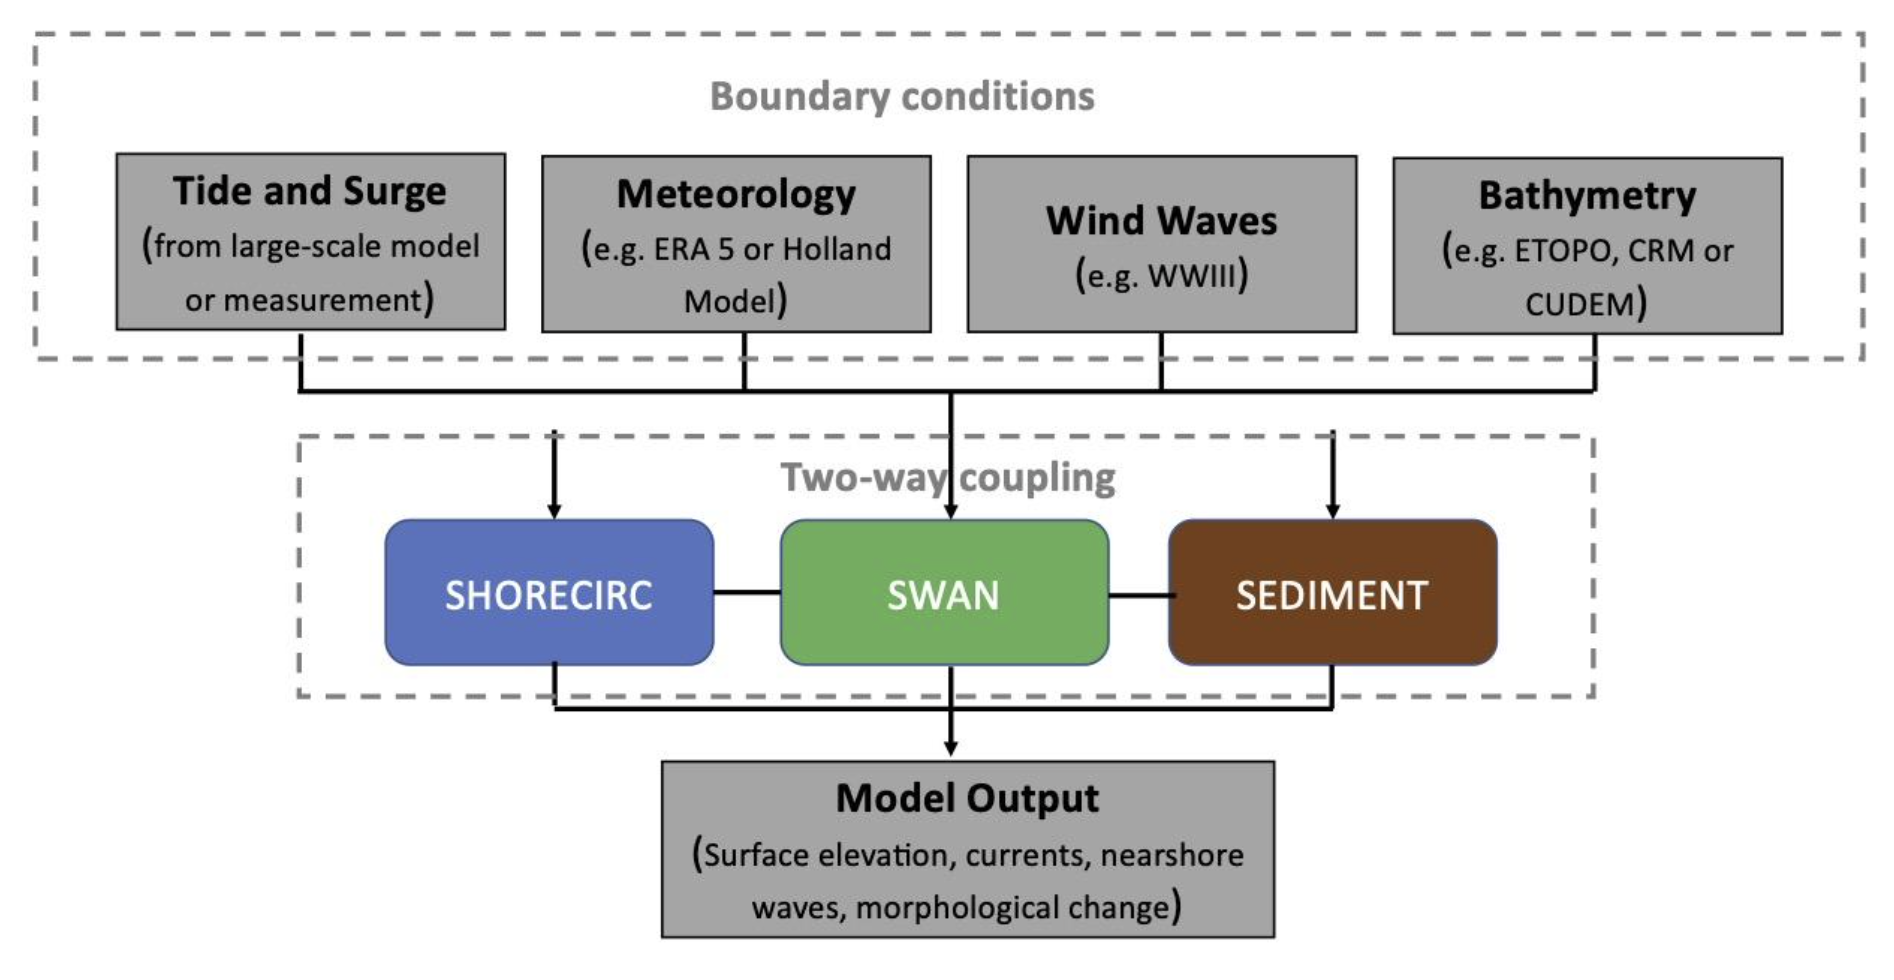
\includegraphics[width=\textwidth]{./figures/nearcom_chart.png}
\caption{The model coupling framework in NEARCOM-TVD. }
\label{nearcom_chart.}
\centering
\end{figure}

\subsection*{8.6.1 Selection of wave and circulation modules in NEARCOM}

\begin{figure}
\centering
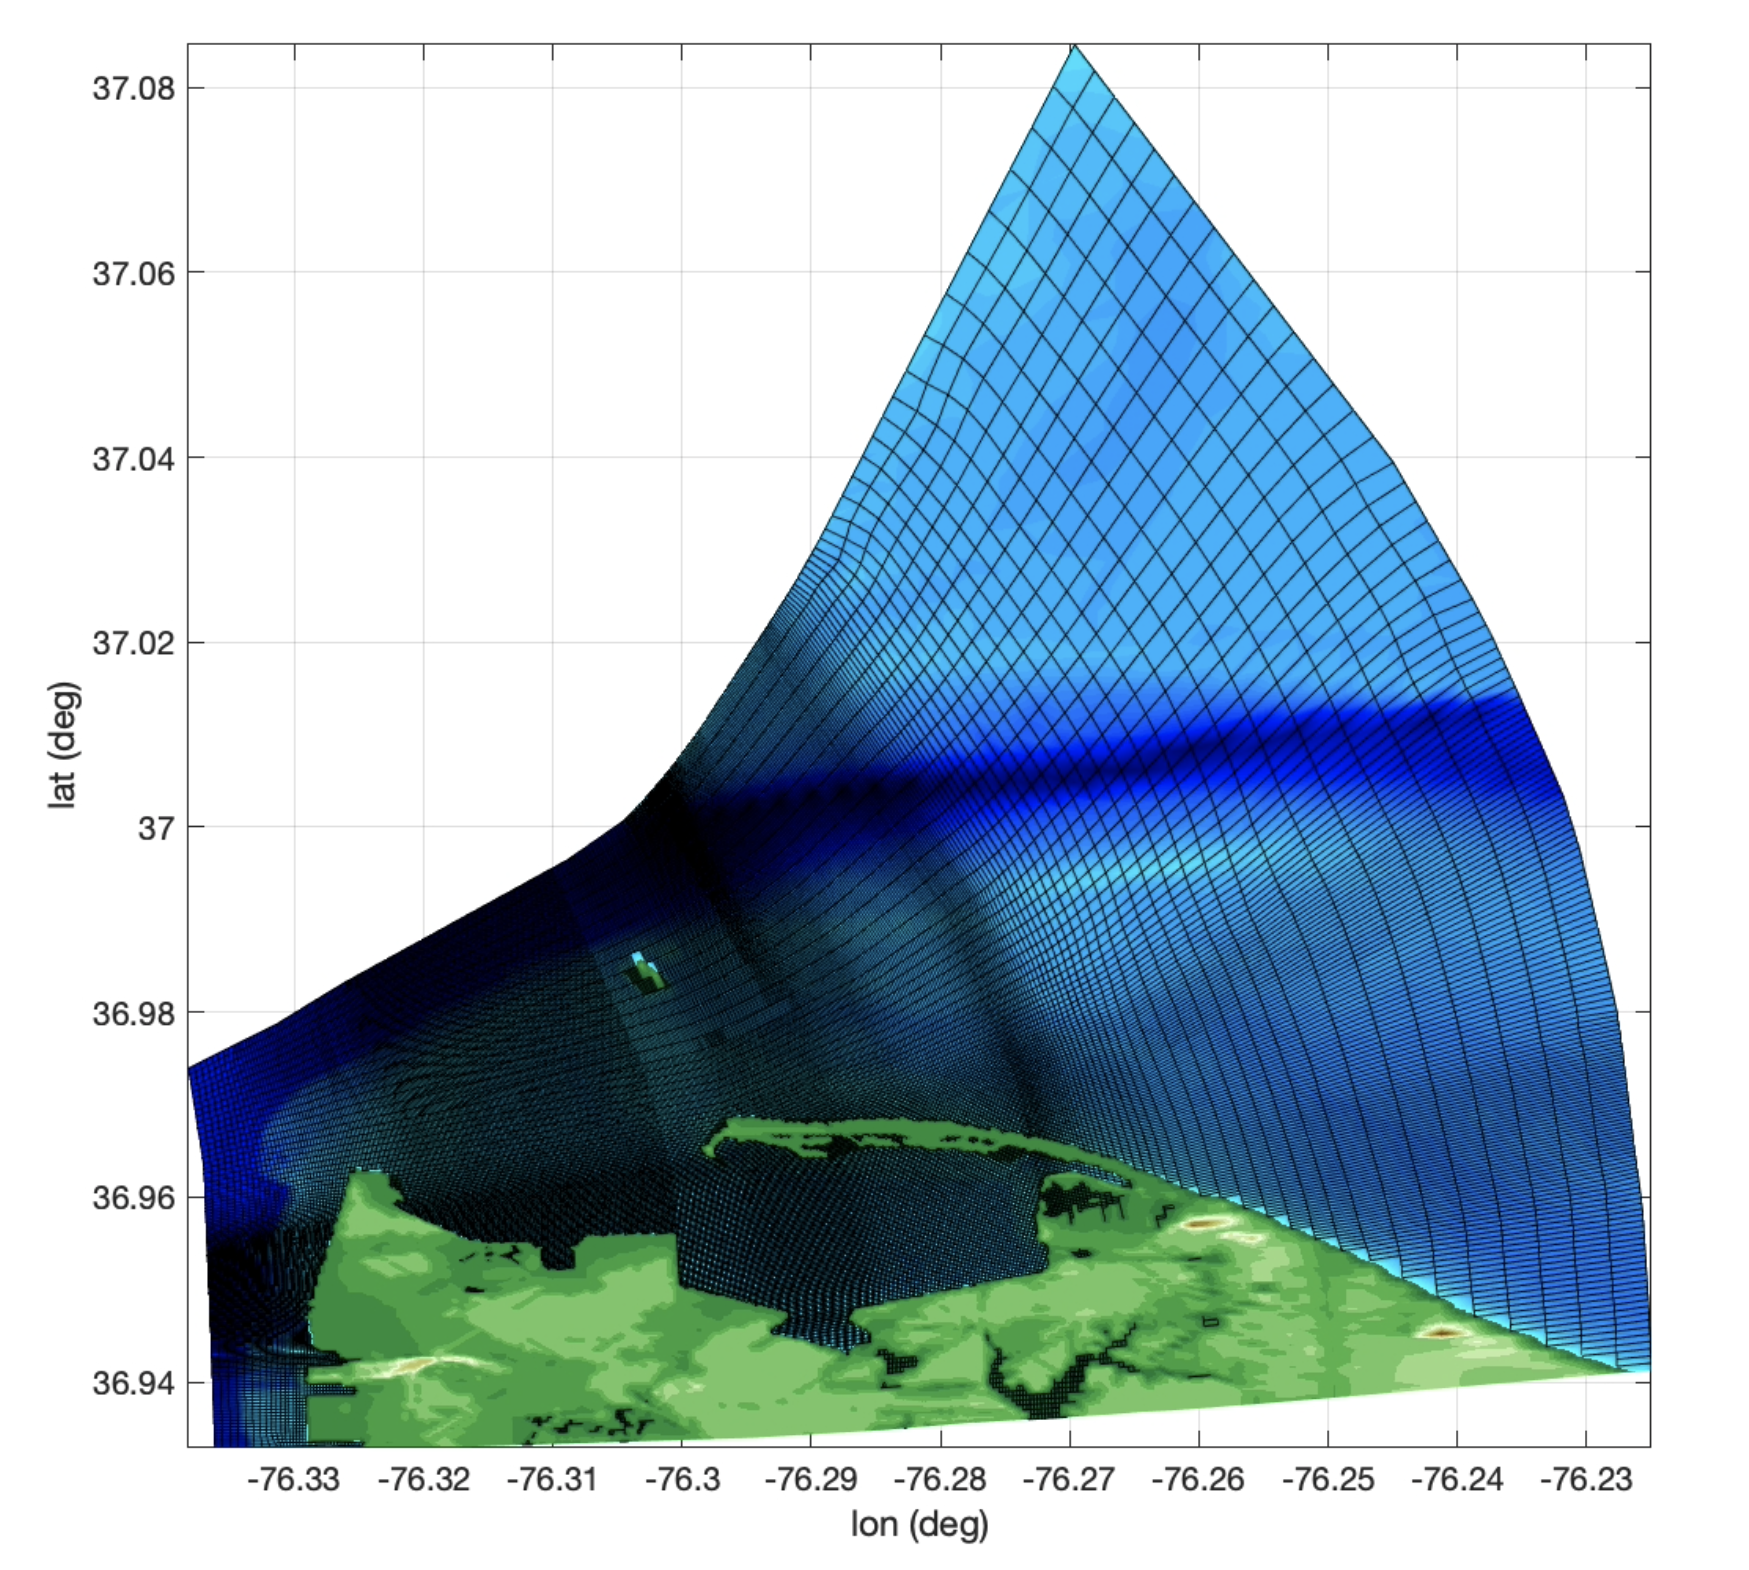
\includegraphics[width=\textwidth]{./figures/nearcom_grid.png}
\caption{Computational grid of NEARCOM. The bathymetry is indicated by colors.}
\label{boundary}
\centering
\end{figure}

In this demonstration study, we applied the combination of the wave model SWAN and the nearshore circulation model SHORECIRC. The coupled SWAN-SHORECIRC model is also called NearCoM-TVD, which was developed using a hybrid finite-difference finite-volume TVD-type scheme on a generalized curvilinear grid. SWAN and SHORECIRC are tightly coupled using the coupler, MASTER Program in the MPI-based parallel computing framework. SWAN calculates wind waves and provides SHORECIRC with radiation stresses to get wave setups and nearshore circulation. The current effects on waves are computed in SWAN with the current input from SHORECIRC.
The model coupling framework is illustrated in Figure 9. Note that the sediment transport module was not applied in the demonstration.

\subsection*{8.6.2 NEARCOM setup}

Figure 10 shows the generalized curvilinear grid with the fine grid resolution at Naval Station Norfolk.
NearCom addresses the nearshore processes only and thus the computational domain is smaller than that used for D-Flow FM or ADCIRC in a typical tide-surge simulation. The tidal and surge boundary conditions for NearCom are provided by a large-scale model, such as D-Flow FM or ADCIRC. The data format for the boundary conditions is (time, elevation, <velocity>), where <velocity> represents depth-averaged current velocity components and are optional.
The original Holland model (Holland, 1980) was implemented in NearCom to model wind/pressure forcing in storm surge simulations. The model also has an optional wind/pressure input which can come from large-scale models. In most NearCom applications for storm events, the wind/pressure data are provided by a large-scale model, consistent with the boundary conditions from the same large-scale model.

\section*{9.3 NEARCOM} 

\subsection*{9.3.1 Selections of scenarios}


\begin{figure}
\centering
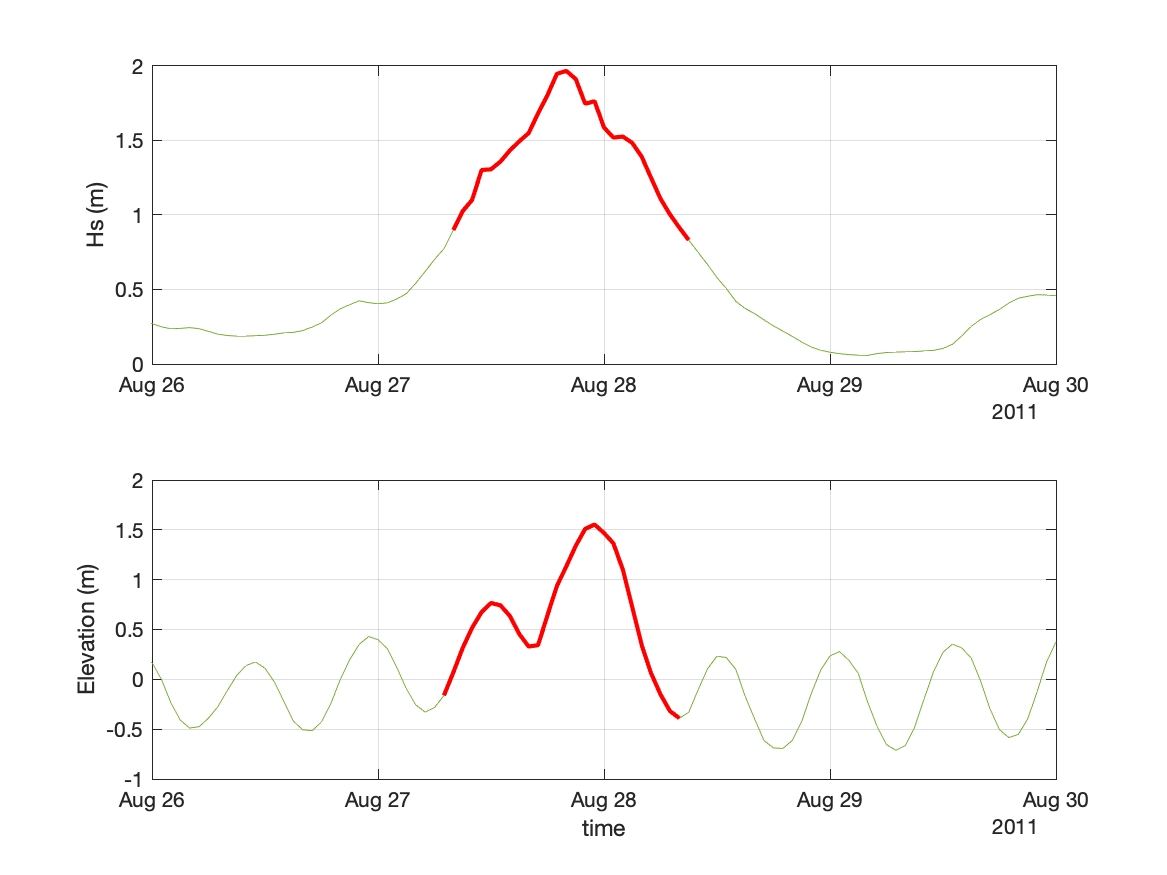
\includegraphics[width=\textwidth]{./figures/nearcom_wave_flow.jpg}
\caption{NEARCOM model input boundary conditions. Time series of significant wave height (top) and surface elevation (bottom) at the boundary point of (36.9742N, 76.2271W). The simulation period is indicated by the red lines. }
\label{ERA5_time}
\centering
\end{figure}

\begin{figure}
\centering
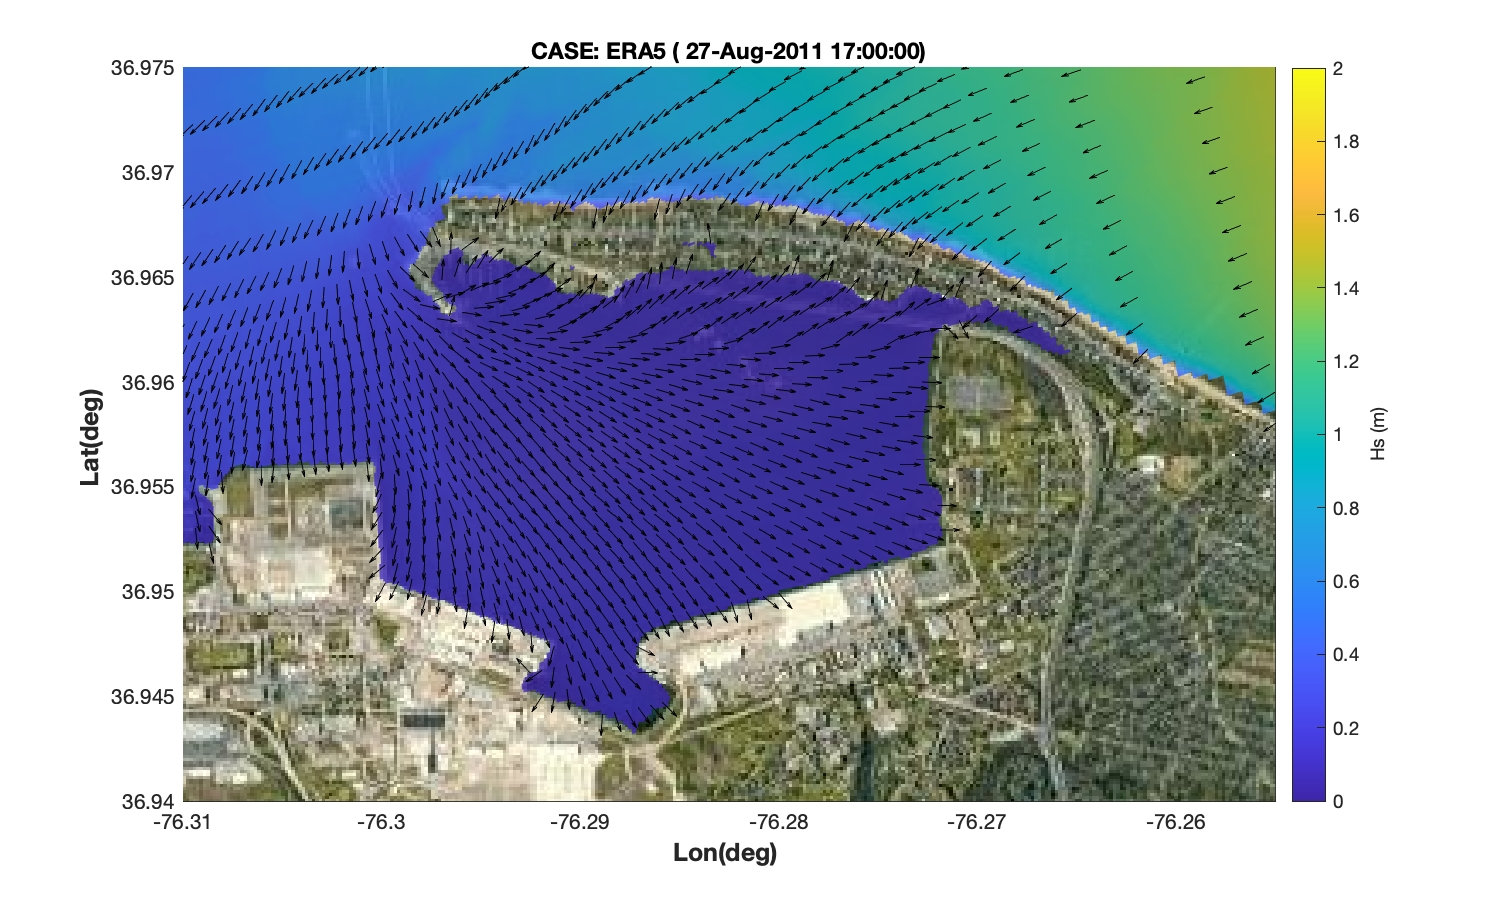
\includegraphics[width=\textwidth]{./figures/nearcom_hs_ERA5_55.jpg}
\caption{Snapshot of wave height distribution (color) and and wave direction (vectors) at the beginning of the storm tide (27-Aug-2011 17:00) for scenario ERA5.}
\label{ERA5_hs_1}
\centering
\end{figure}

\begin{figure}
\centering
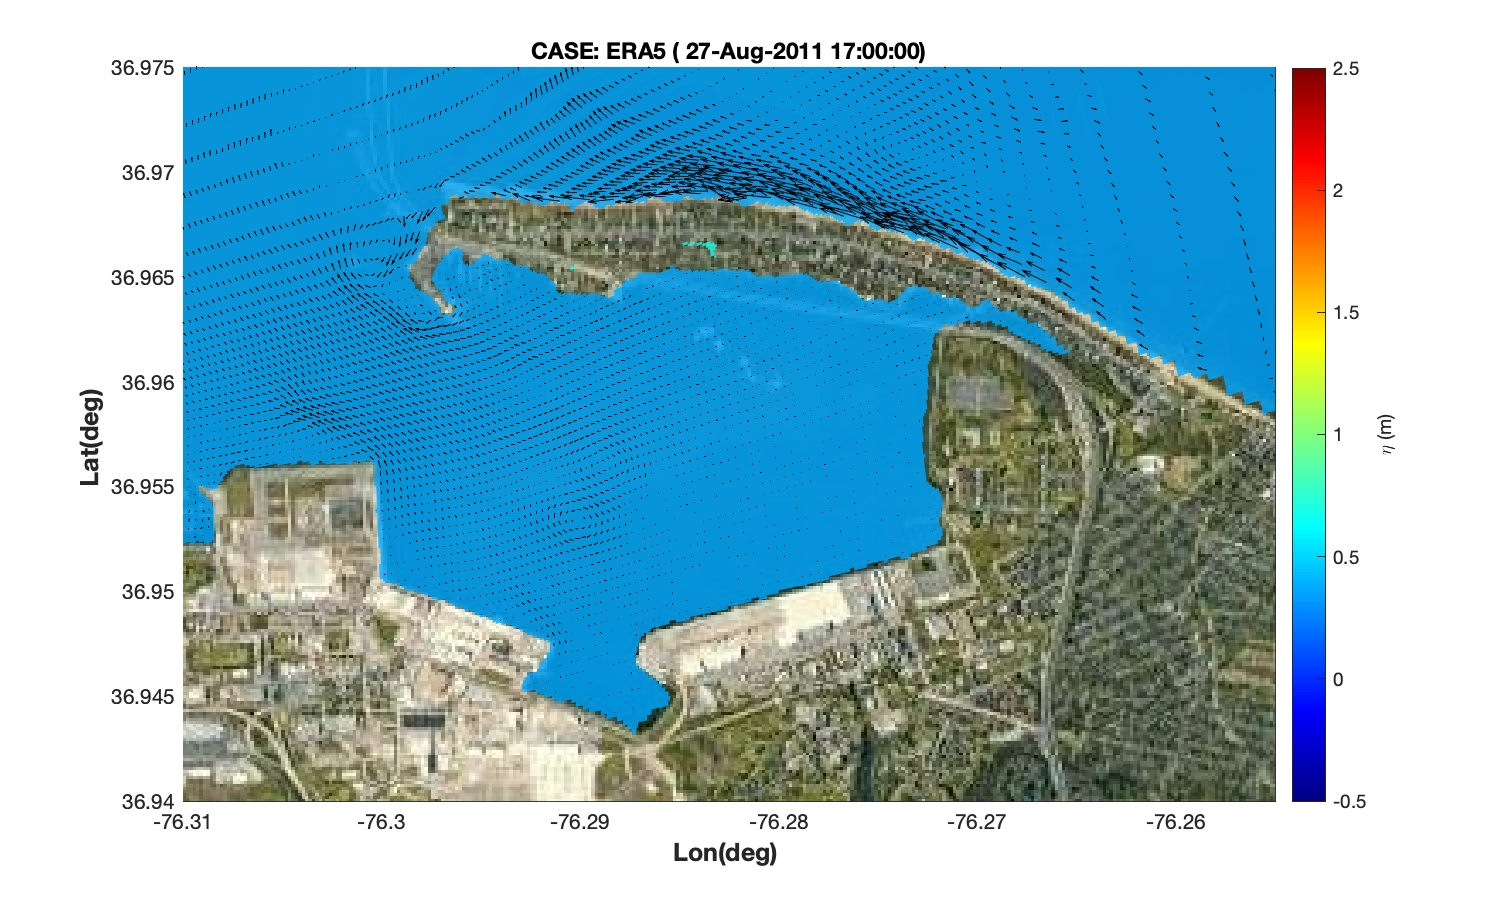
\includegraphics[width=\textwidth]{./figures/nearcom_ele_ERA5_55.jpg}
\caption{Snapshot of surface elevation (color) and and currents (vectors) at the beginning of the storm tide (27-Aug-2011 17:00) for scenario ERA5.}
\label{ERA5_eta_1}
\centering
\end{figure}

\begin{figure}
\centering
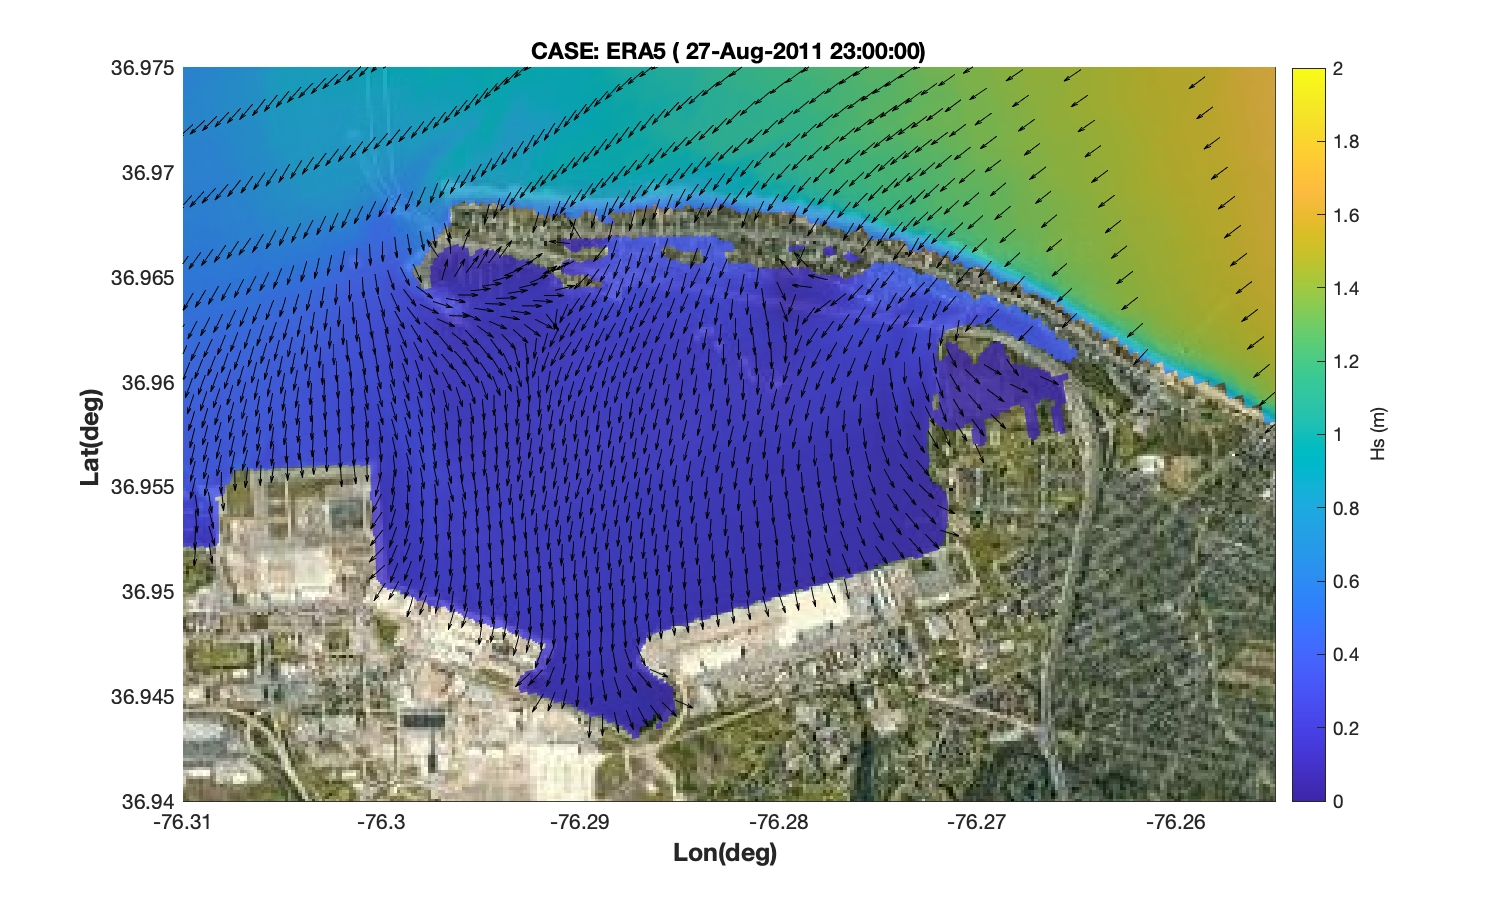
\includegraphics[width=\textwidth]{./figures/nearcom_hs_ERA5_91.jpg}
\caption{Snapshot of wave height distribution (color) and and wave direction (vectors) at the peak of the storm tide (27-Aug-2011 23:00) for scenario ERA5. }
\label{ERA5_hs_2}
\centering
\end{figure}

\begin{figure}
\centering
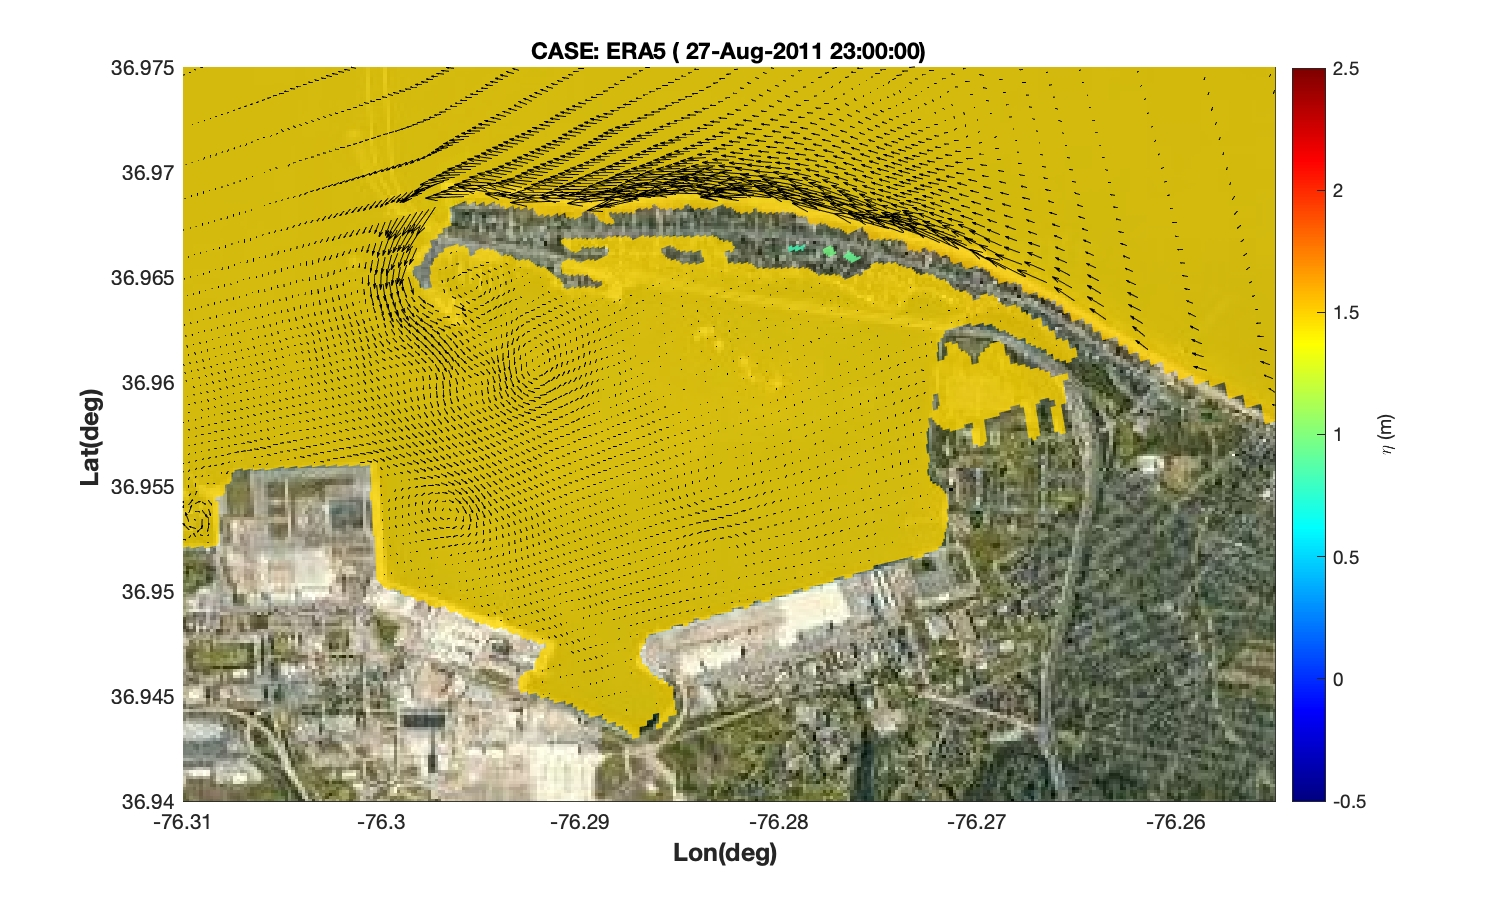
\includegraphics[width=\textwidth]{./figures/nearcom_ele_ERA5_91.jpg}
\caption{Snapshot of surface elevation (color) and and currents (vectors) at the peak of the storm tide (27-Aug-2011 23:00) for scenario ERA5.}
\label{ERA5_eta_2}
\centering
\end{figure}

\begin{figure}
\centering
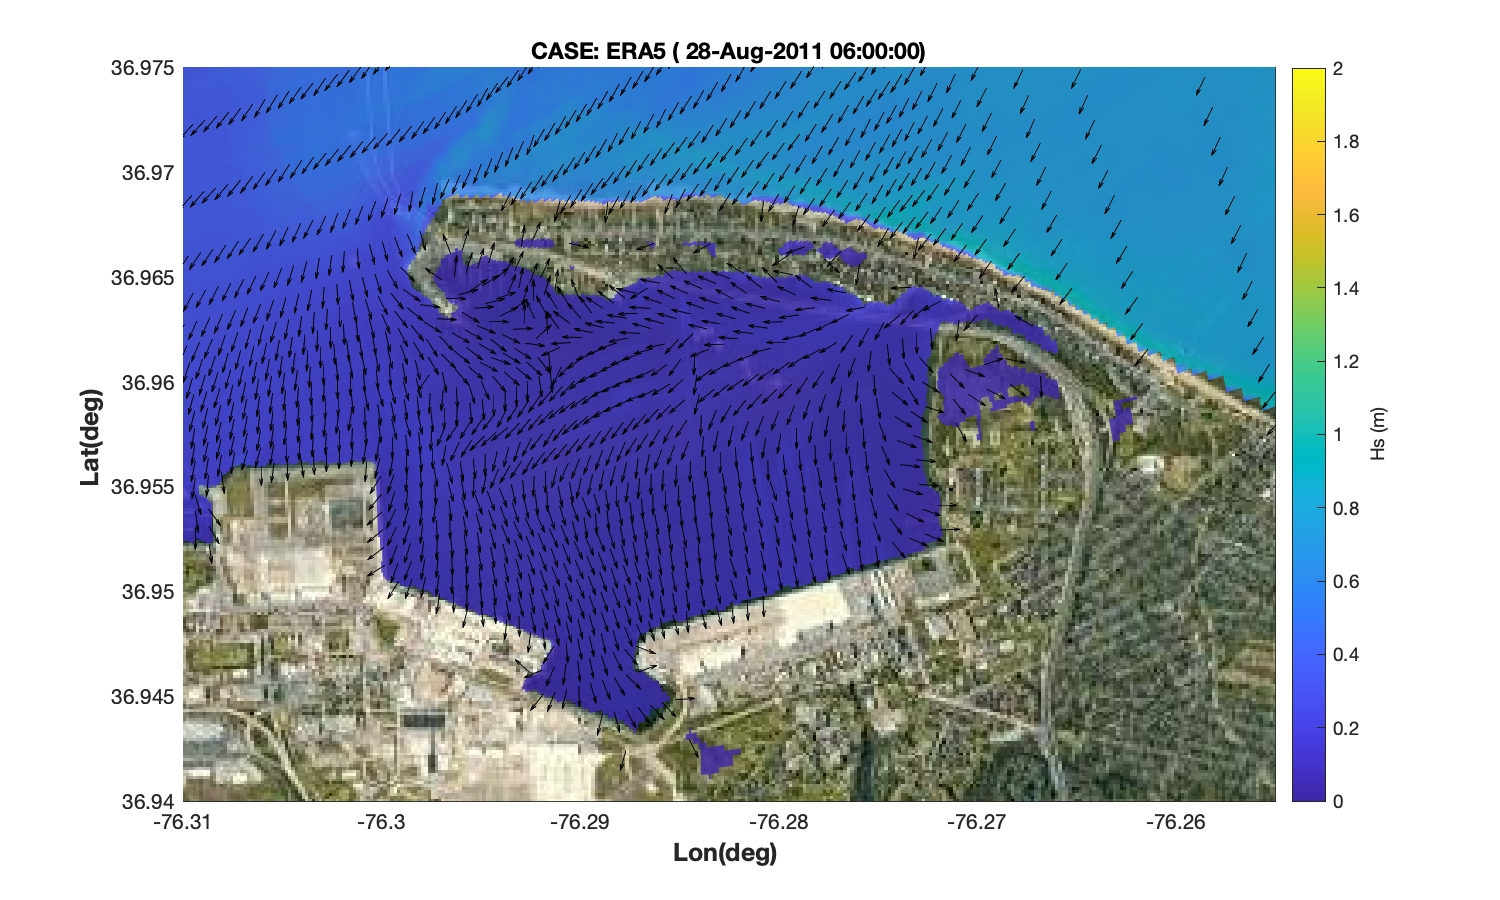
\includegraphics[width=\textwidth]{./figures/nearcom_hs_ERA5_133.jpg}
\caption{Snapshot of wave height distribution (color) and and wave direction (vectors) at the low storm tide (28-Aug-2011 06:00) for scenario ERA5. }
\label{ERA5_hs_3}
\centering
\end{figure}

\begin{figure}
\centering
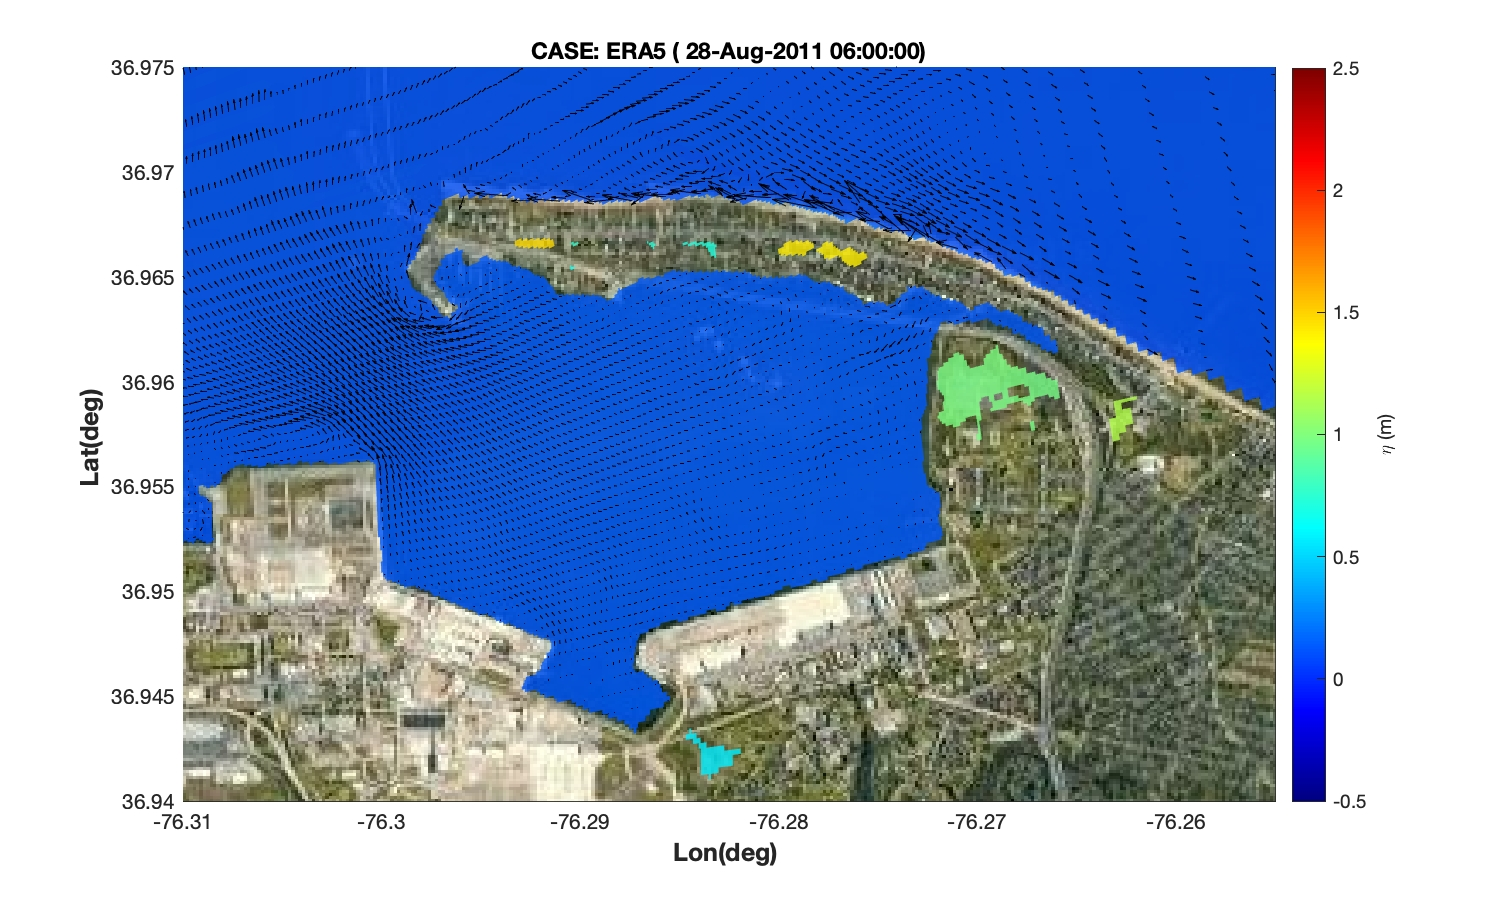
\includegraphics[width=\textwidth]{./figures/nearcom_ele_ERA5_133.jpg}
\caption{Snapshot of surface elevation (color) and and currents (vectors) at the low storm tide (28-Aug-2011 06:00) for scenario ERA5. }
\label{ERA5_eta_3}
\centering
\end{figure}

% wave versus no wave

\begin{figure}
\centering
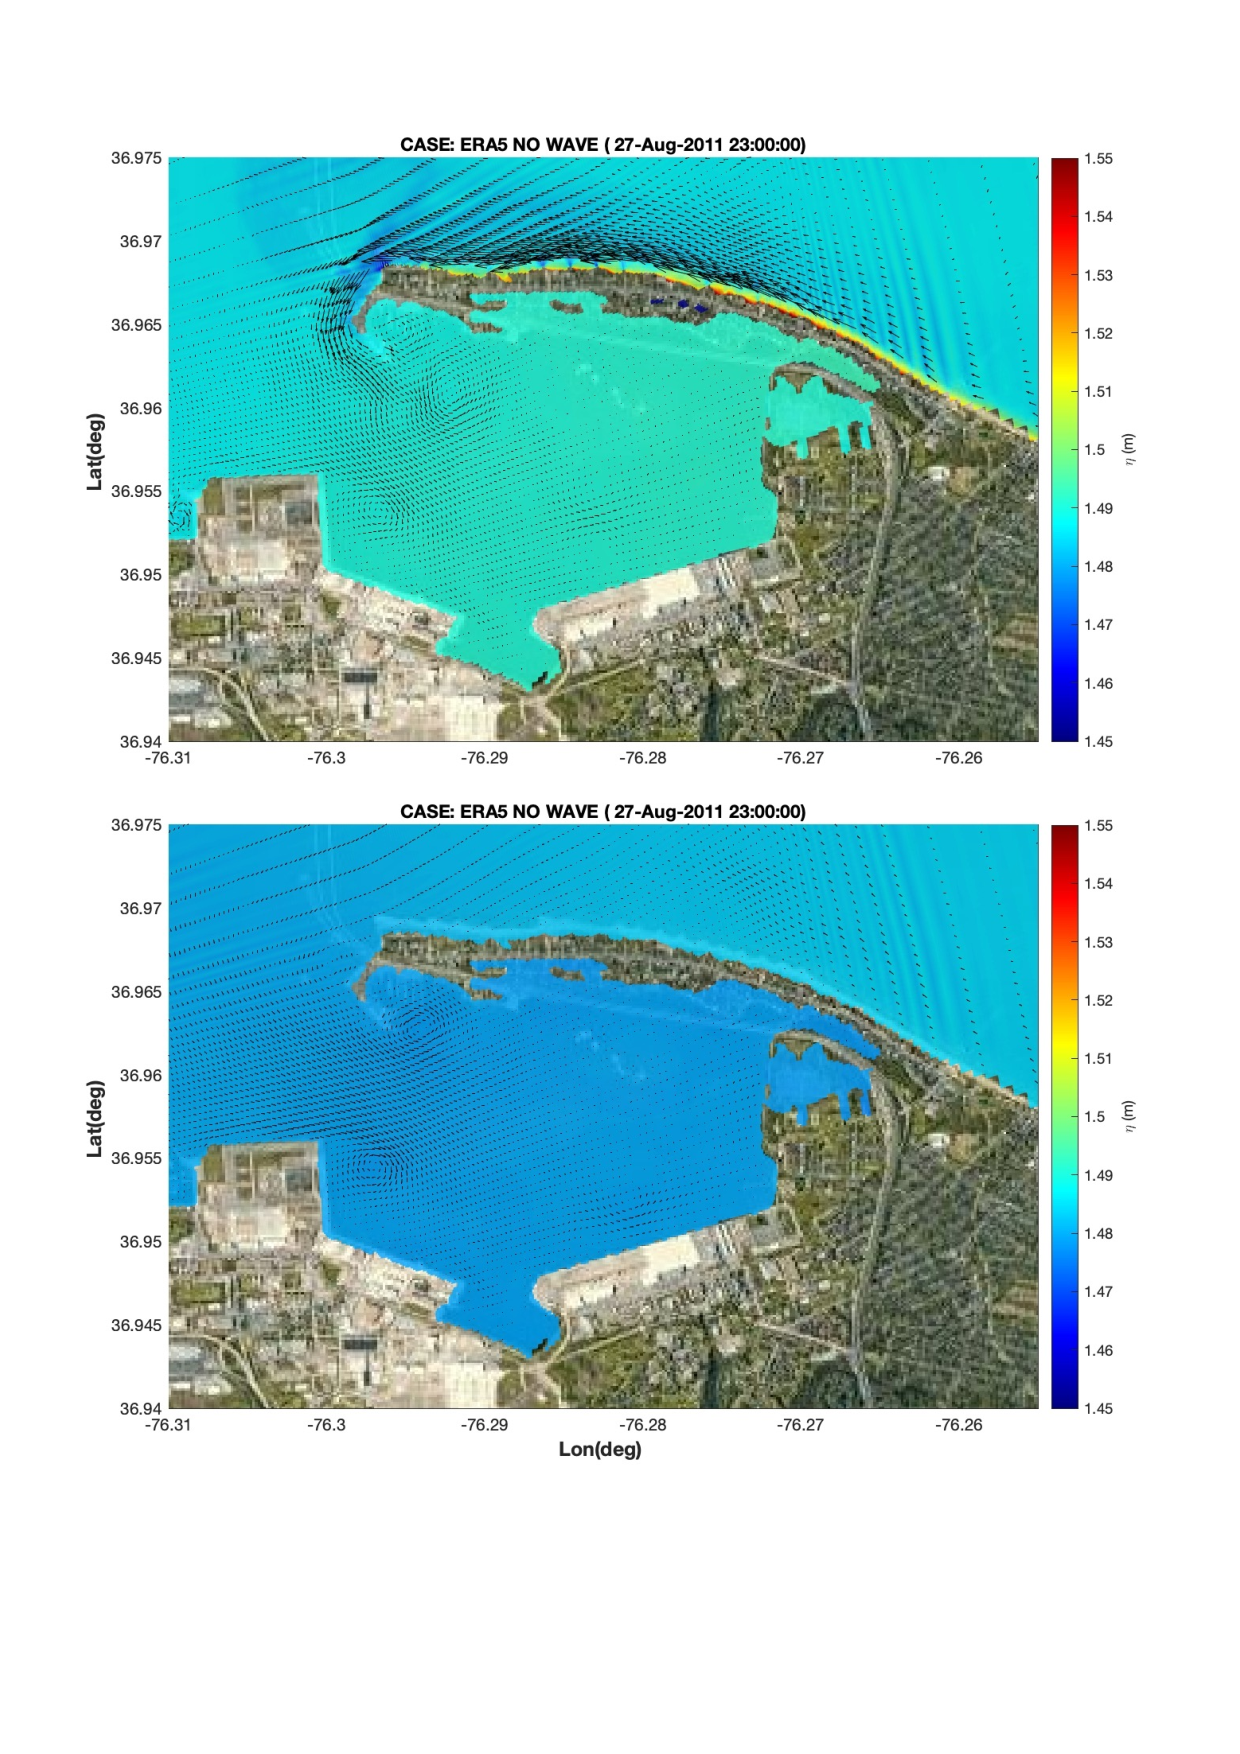
\includegraphics[width=\textwidth]{./figures/nearcom_wo_wave.pdf}
\caption{Comparison of surface elevation and currents at the peak storm tide between models with and without the wave module coupled in the NEARCOM system.}
\label{ERA5_eta_wo_wave}
\centering
\end{figure}


\begin{figure}
\centering
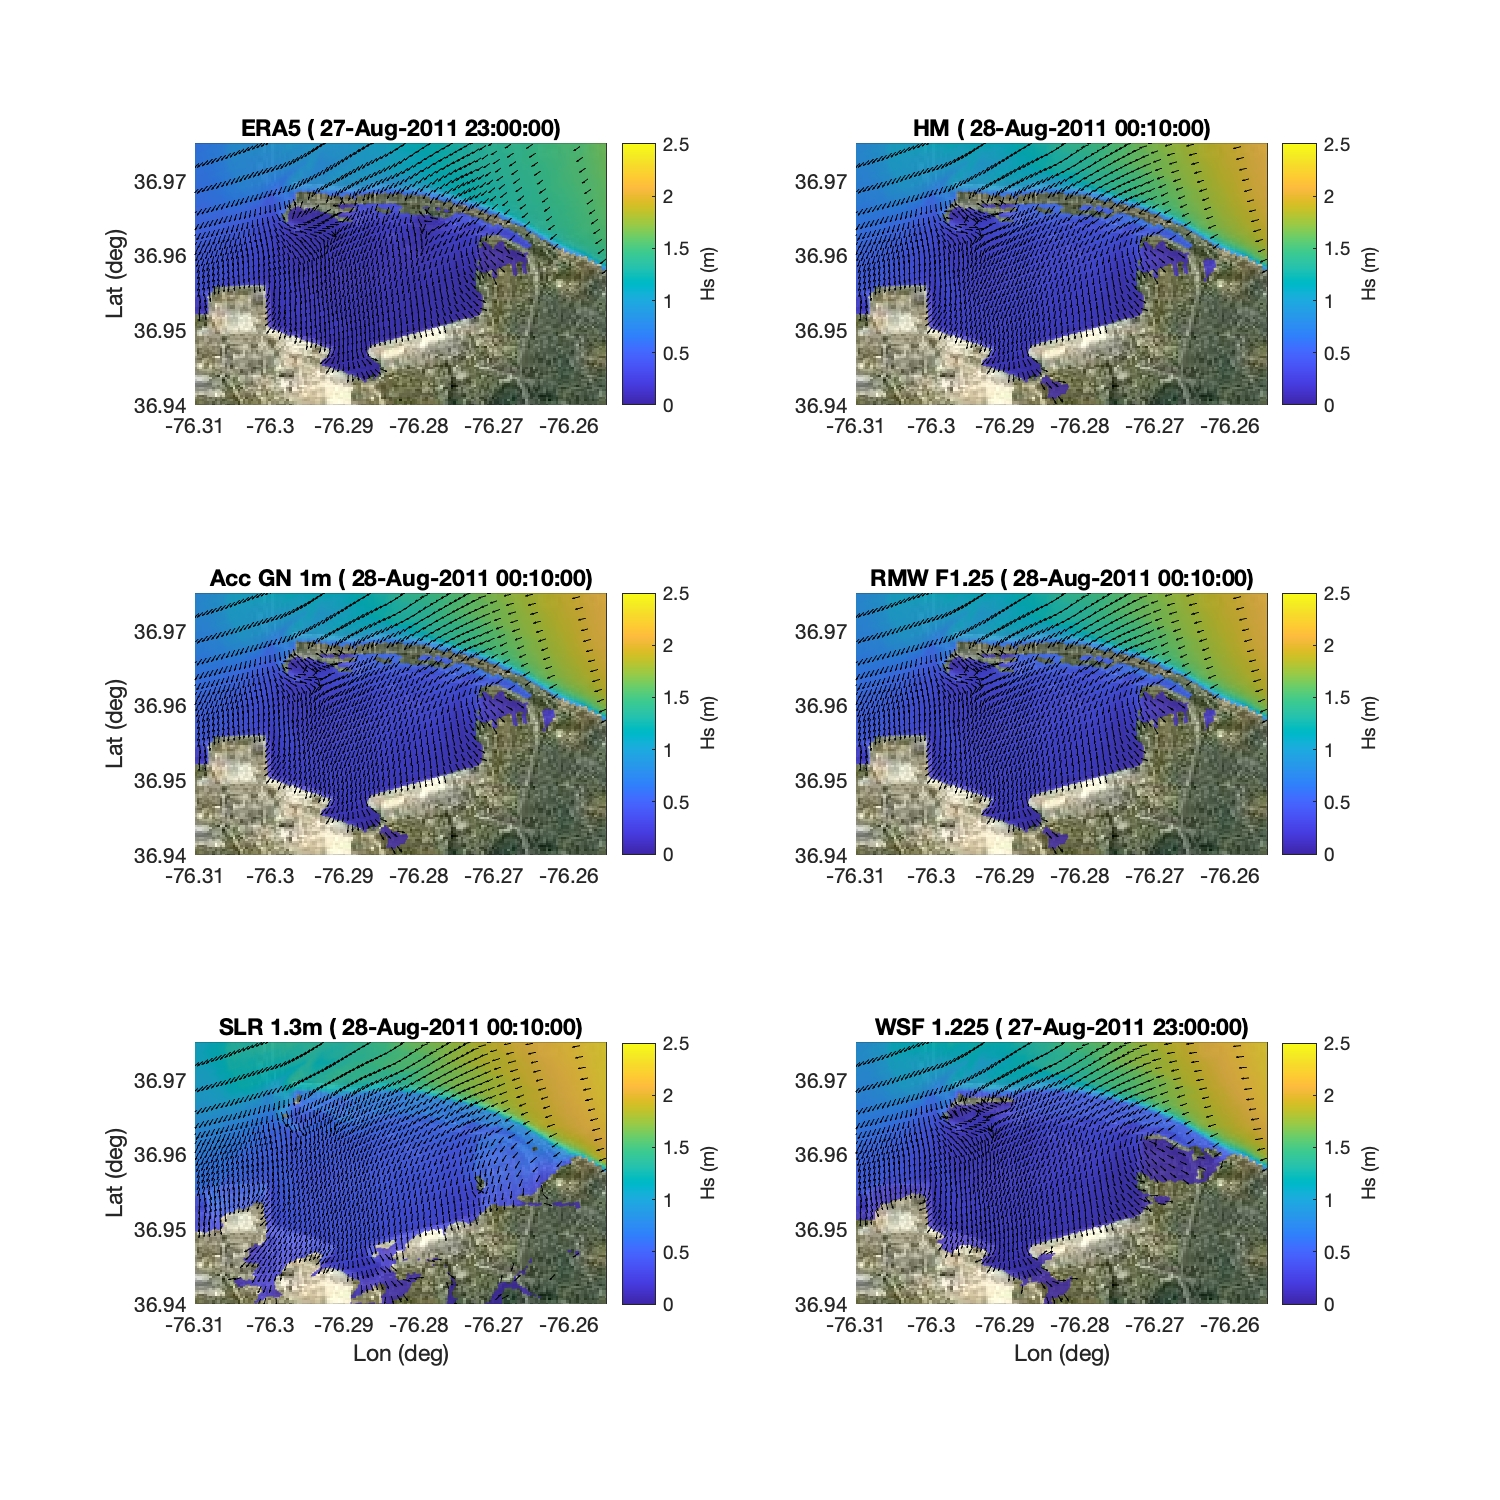
\includegraphics[width=\textwidth]{./figures/nearcom_hs.jpg}
\caption{NEARCOM results of significant wave height (color) and wave direction (vectors) at the peak storm tide from the six selected scenarios.}
\label{nearcom_6_cases_hs}
\centering
\end{figure}

\begin{figure}
\centering
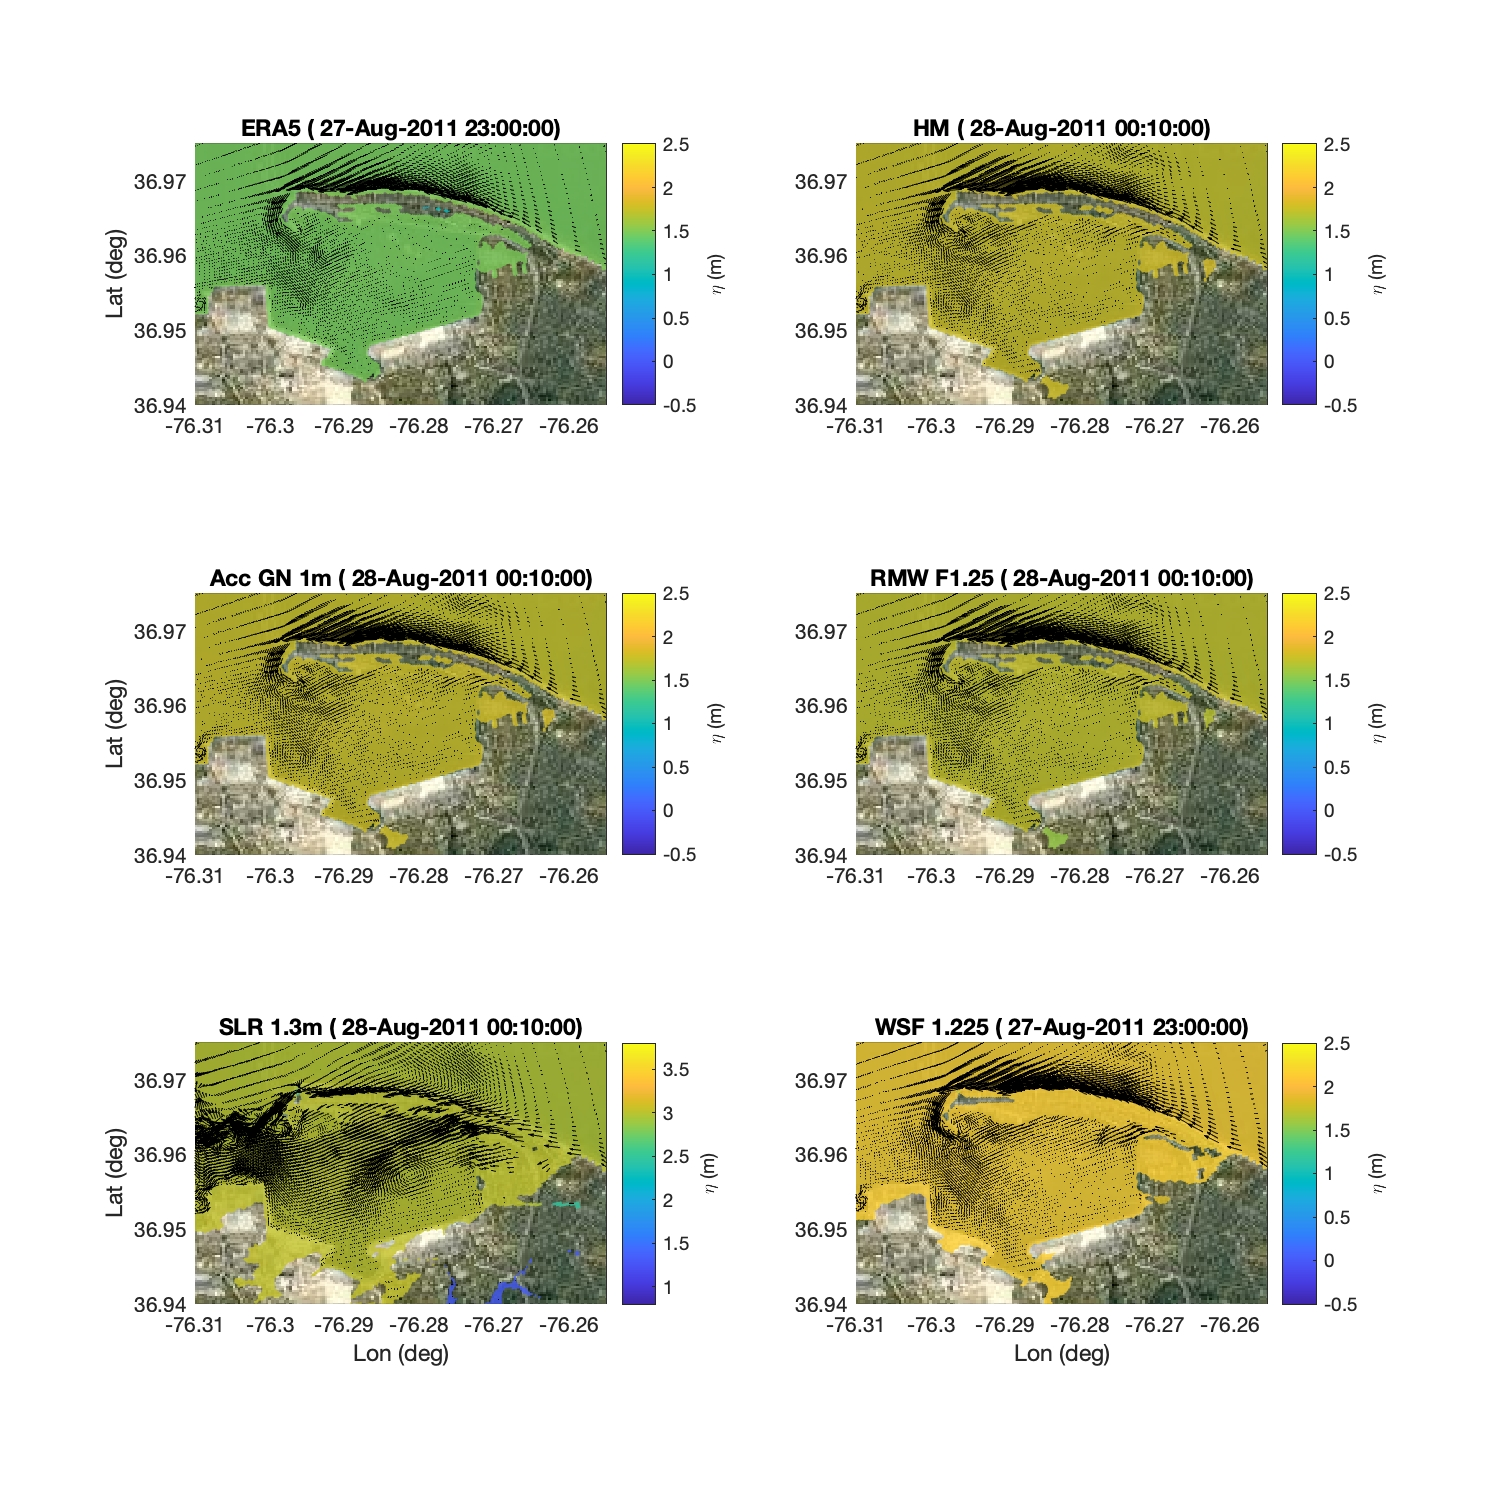
\includegraphics[width=\textwidth]{./figures/nearcom_eta_uv.jpg}
\caption{NEARCOM results of surface elevation (color) and currents (vectors) at the peak storm tide from the six selected scenarios}
\label{nearcom_6_cases_eta}
\centering
\end{figure}

\begin{figure}
\centering
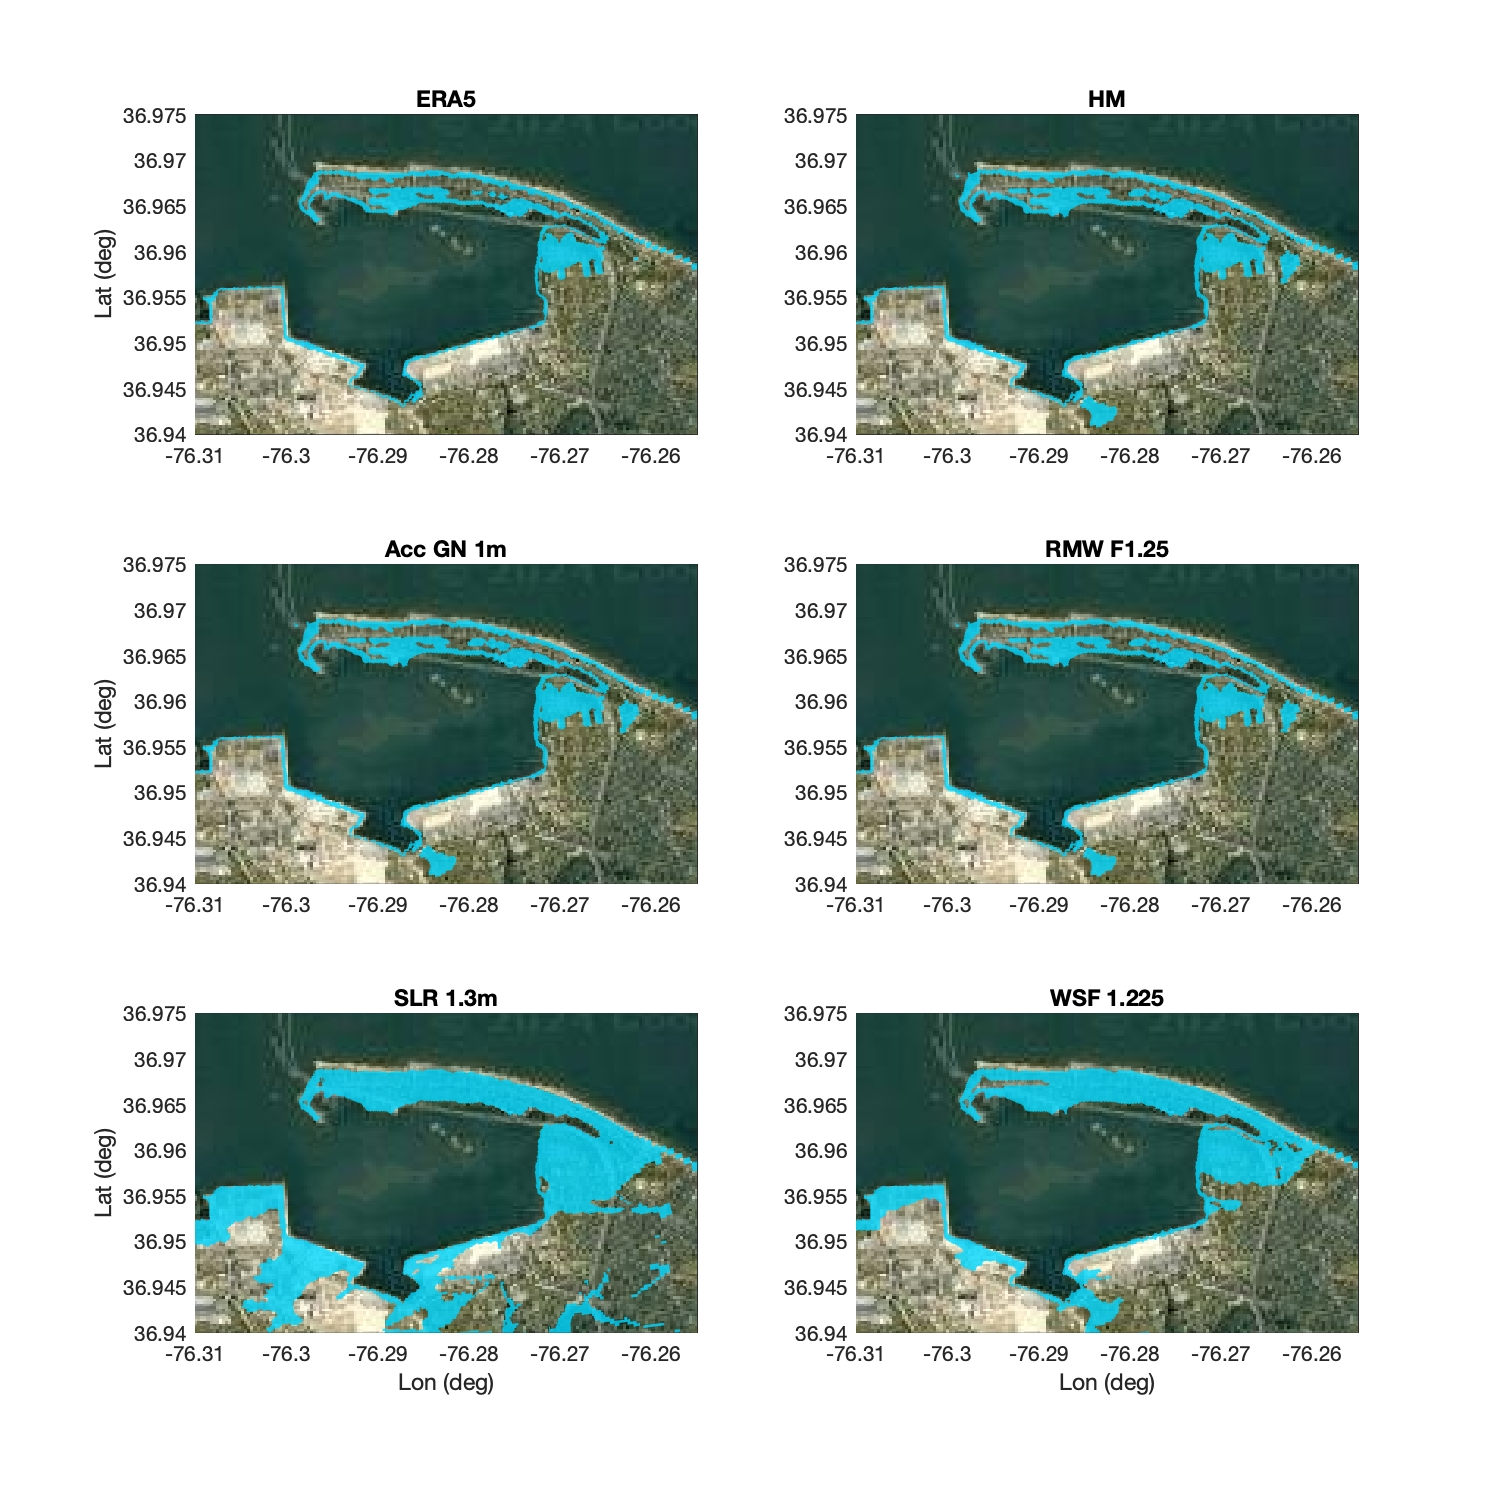
\includegraphics[width=\textwidth]{./figures/nearcom_flood.jpg}
\caption{NEARCOM results of flooded area (blue color) from the six selected scenarios.}
\label{nearcom_6_cases_flood}
\centering
\end{figure}

\begin{figure}
\centering
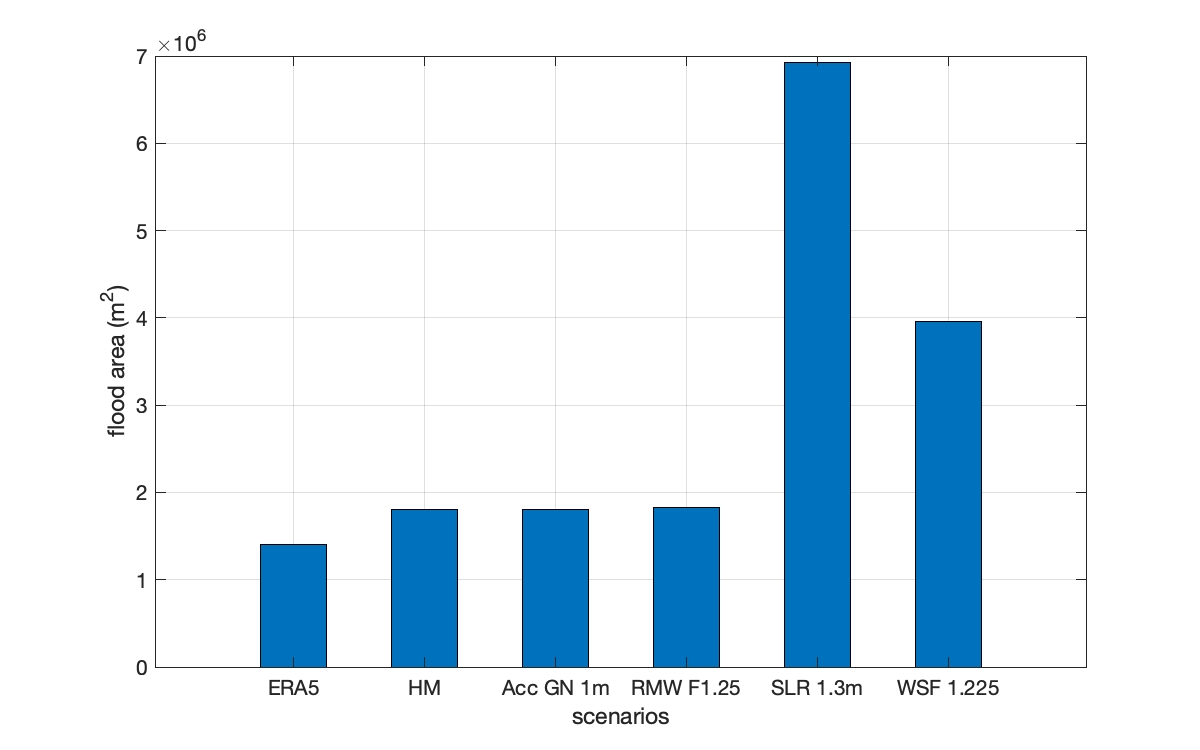
\includegraphics[width=\textwidth]{./figures/nearcom_bars.jpg}
\caption{Flooded areas (m$^2$) in the NEARCOM computational domain from the six selected scenarios.}
\label{nearcom_bars}
\centering
\end{figure}

% funwave

\begin{figure}
\centering
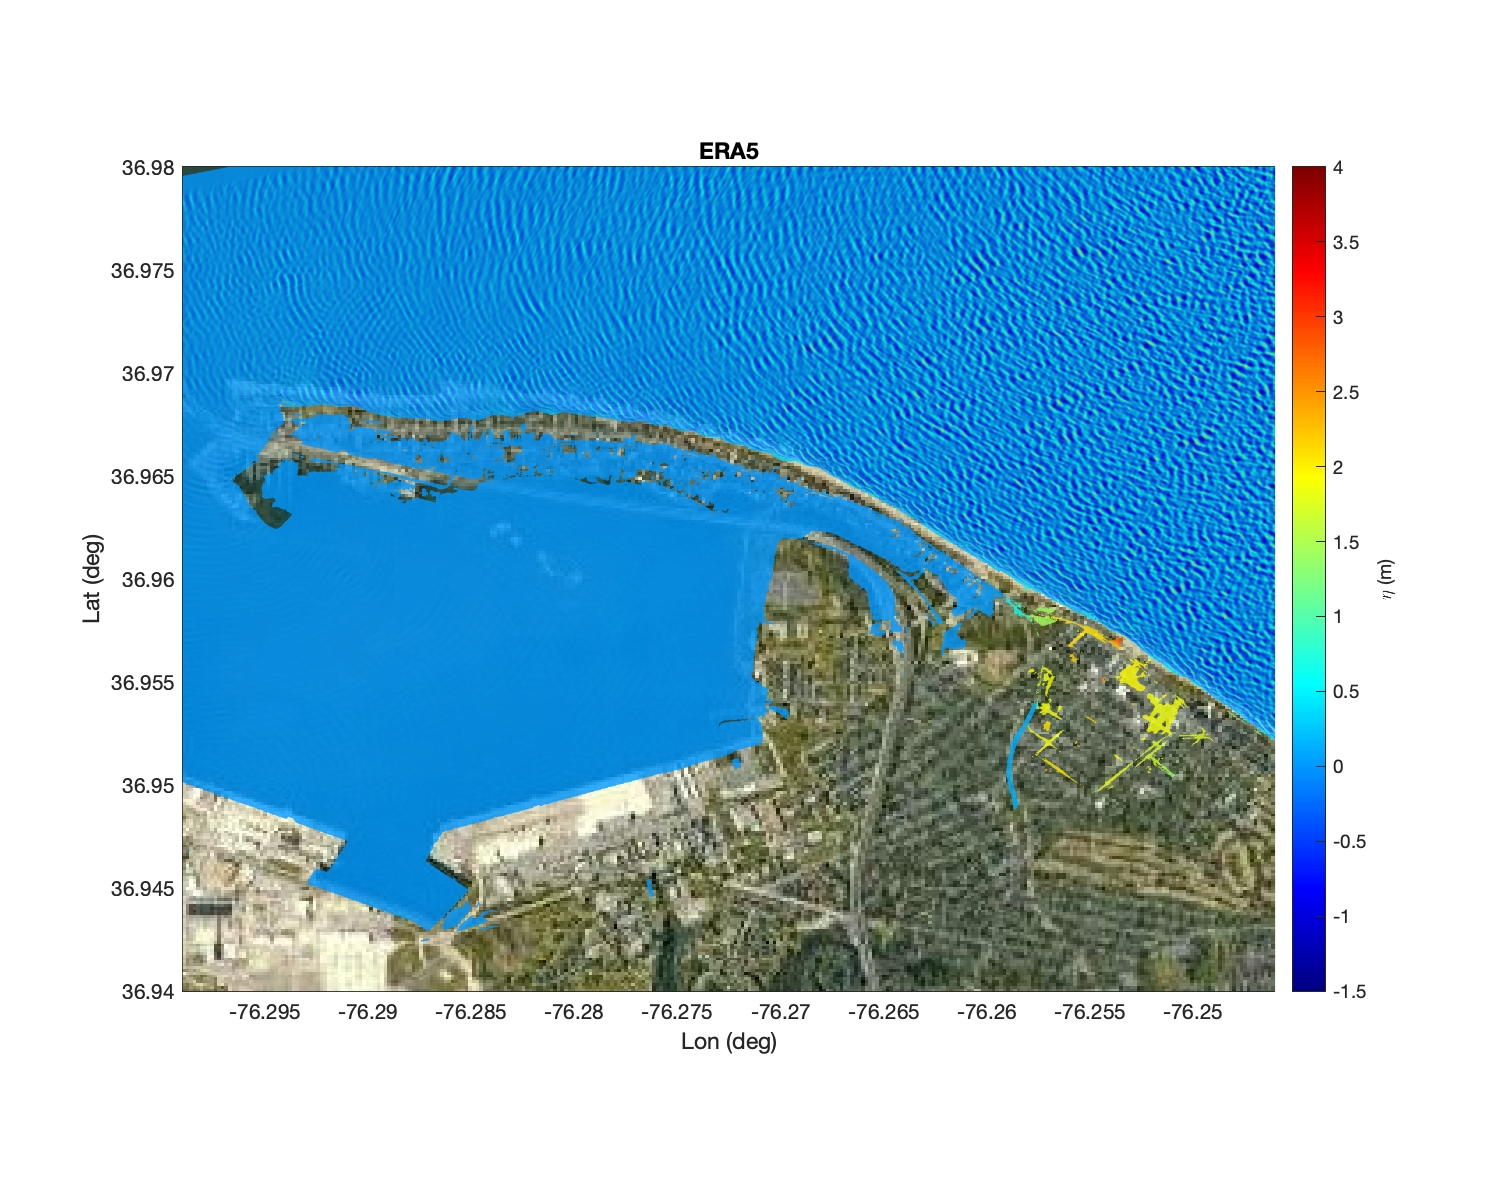
\includegraphics[width=\textwidth]{./figures/funwave_ERA5_eta.jpg}
\caption{Snapshot of wave surface at the peak of the storm tide (27-Aug-2011 23:00) modeled by FUNWAVE-TVD for scenario ERA5. }
\label{funwave_ERA5_eta}
\centering
\end{figure}

\begin{figure}
\centering
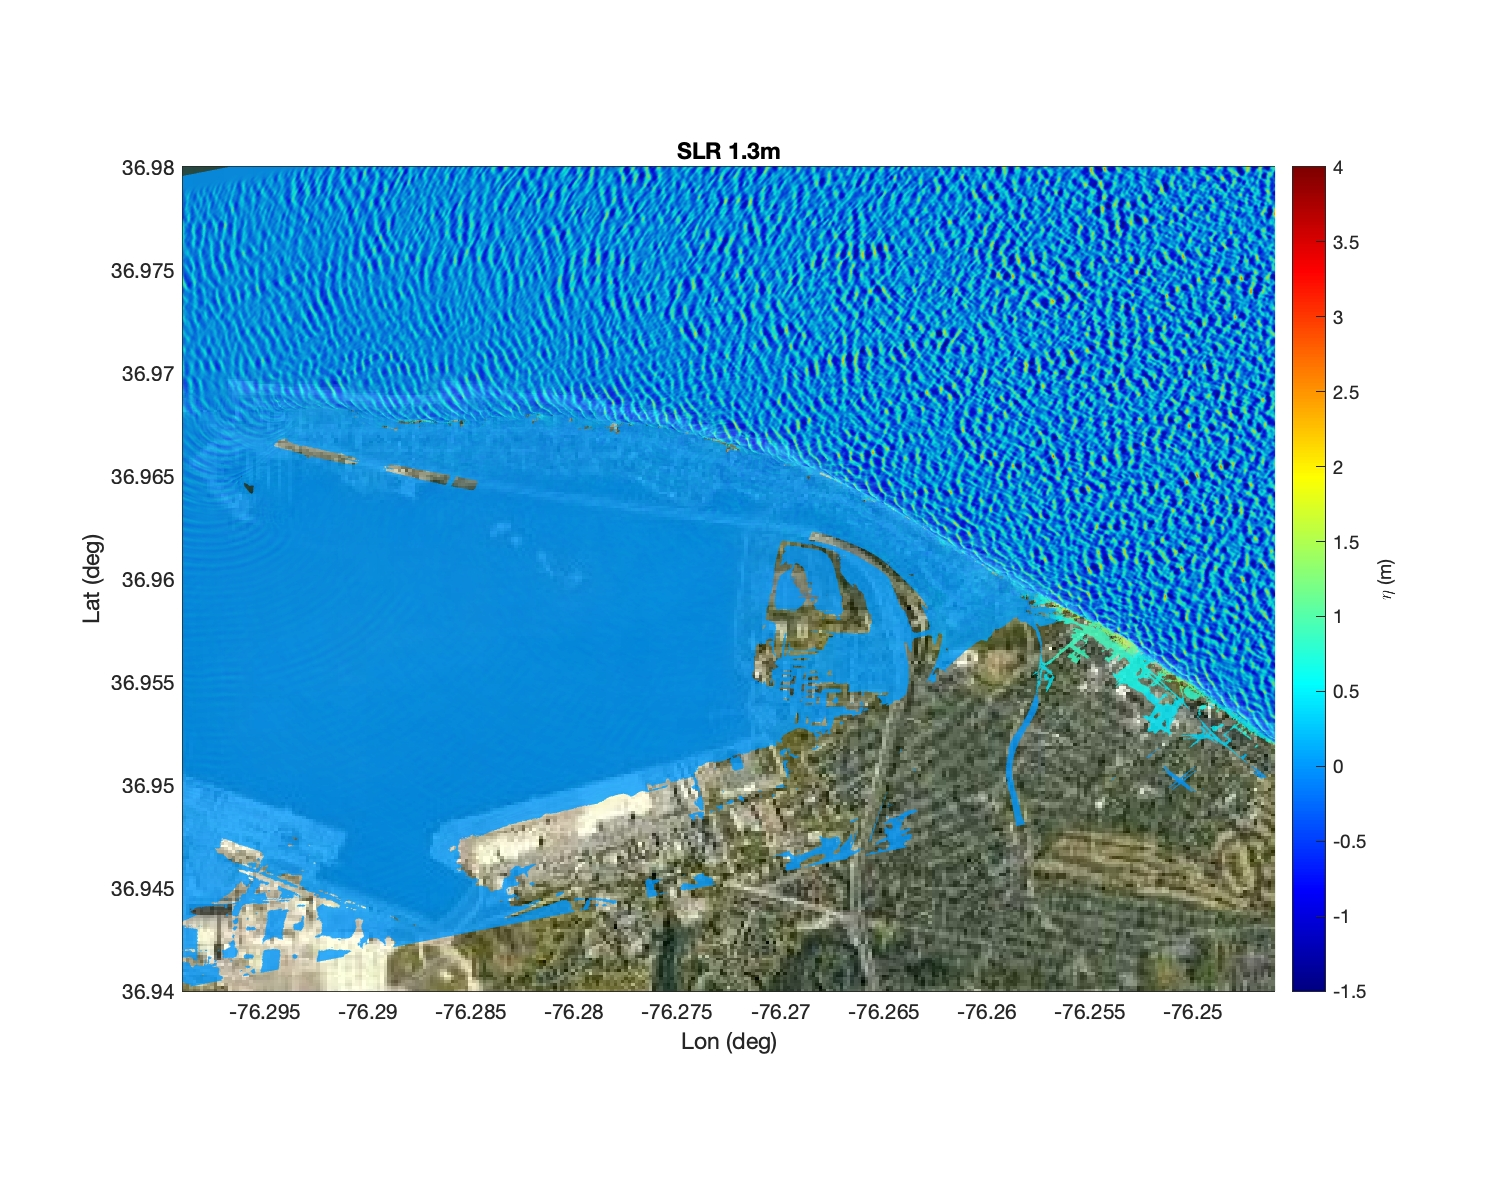
\includegraphics[width=\textwidth]{./figures/funwave_SLR _eta.jpg}
\caption{Snapshot of wave surface at the peak of the storm tide (27-Aug-2011 23:00) modeled by FUNWAVE-TVD for scenario SLR 1.3 m. }
\label{funwave_SLR_eta}
\centering
\end{figure}

\begin{figure}
\centering
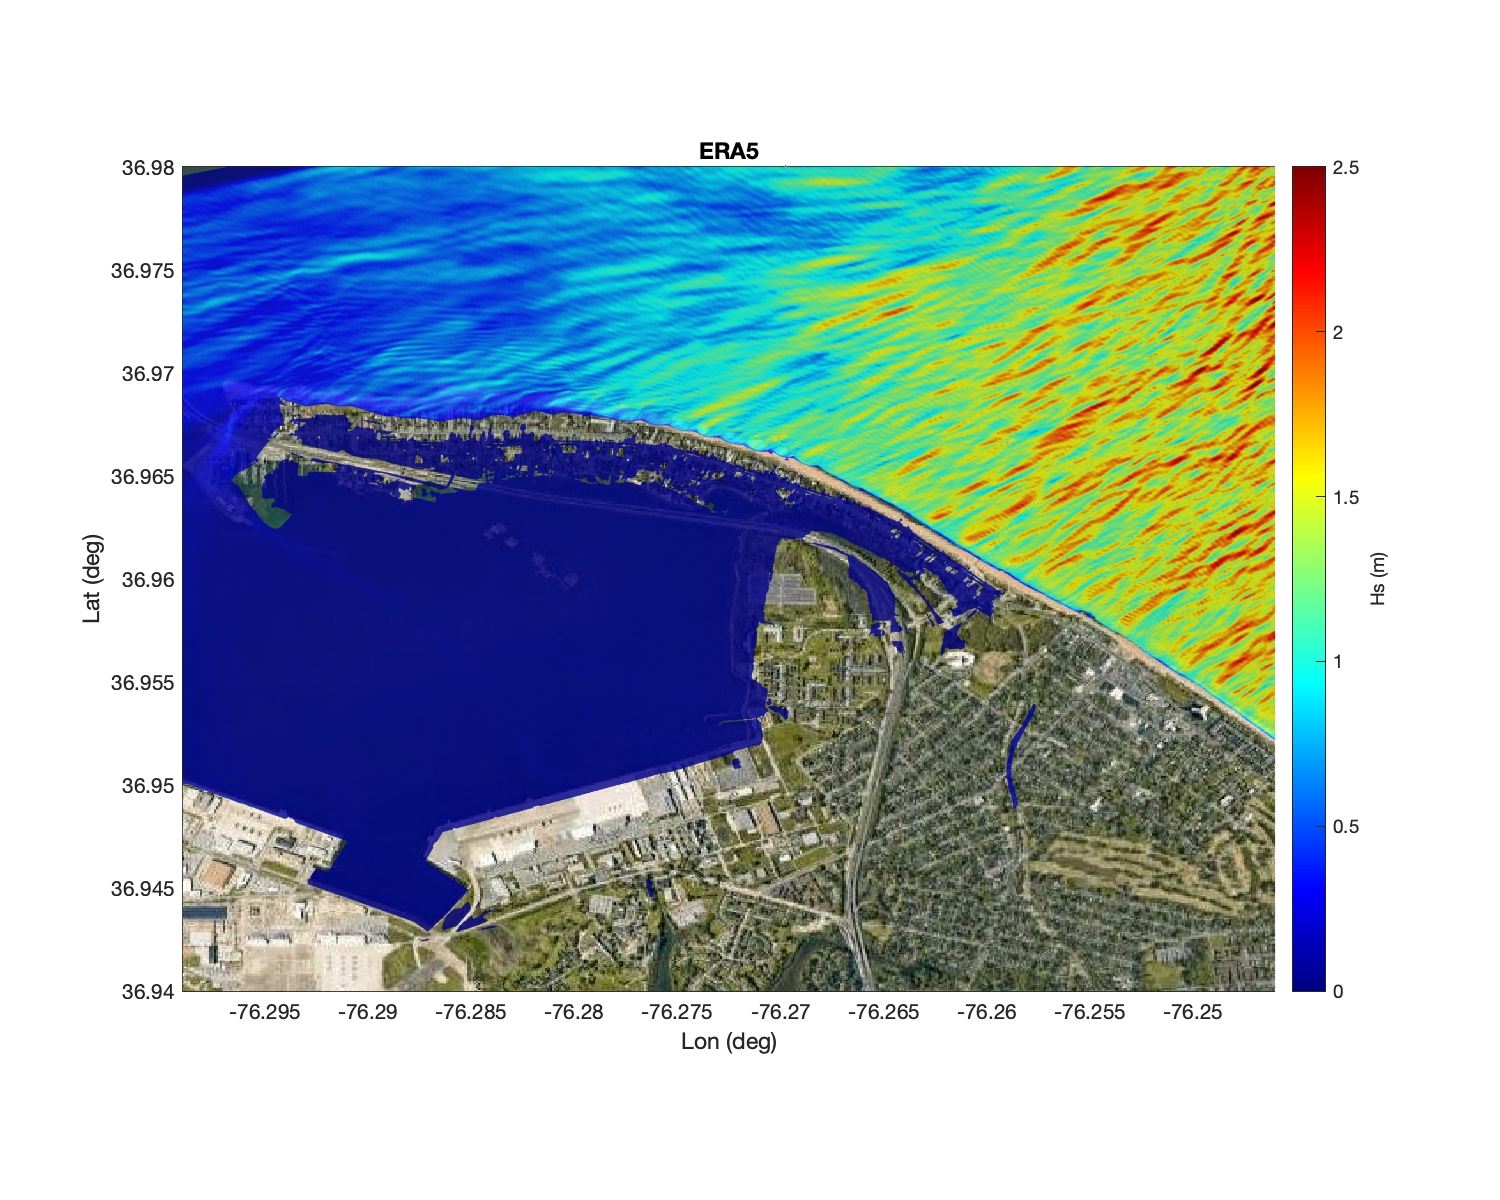
\includegraphics[width=\textwidth]{./figures/funwave_ERA5_hs.jpg}
\caption{FUNWAVE-TVD result of significant wave height at the peak storm tide (27-Aug-2011 23:00) for scenarios ERA5.  }
\label{funwave_ERA5_hs}
\centering
\end{figure}

\begin{figure}
\centering
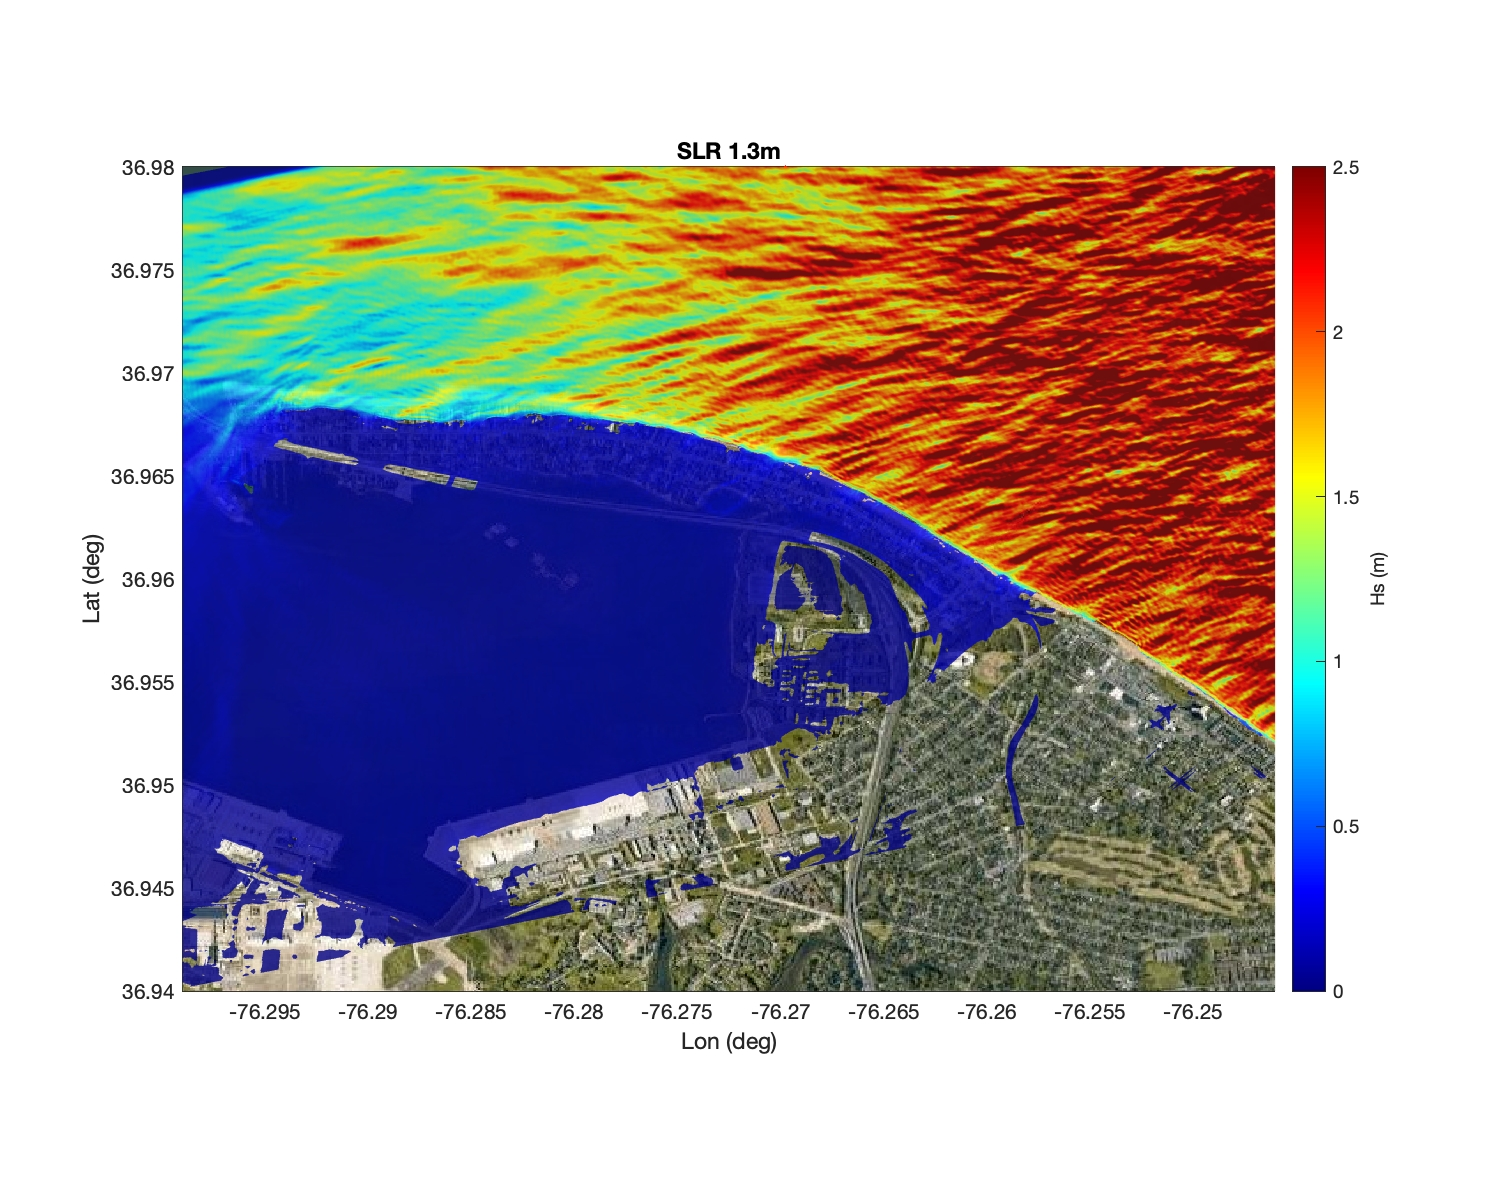
\includegraphics[width=\textwidth]{./figures/funwave_SLR_hs.jpg}
\caption{FUNWAVE-TVD result of significant wave height at the peak storm tide (27-Aug-2011 23:00) for scenarios SLR 1.3 m.  }
\label{funwave_SLR_hs }
\centering
\end{figure}

\begin{figure}
\centering
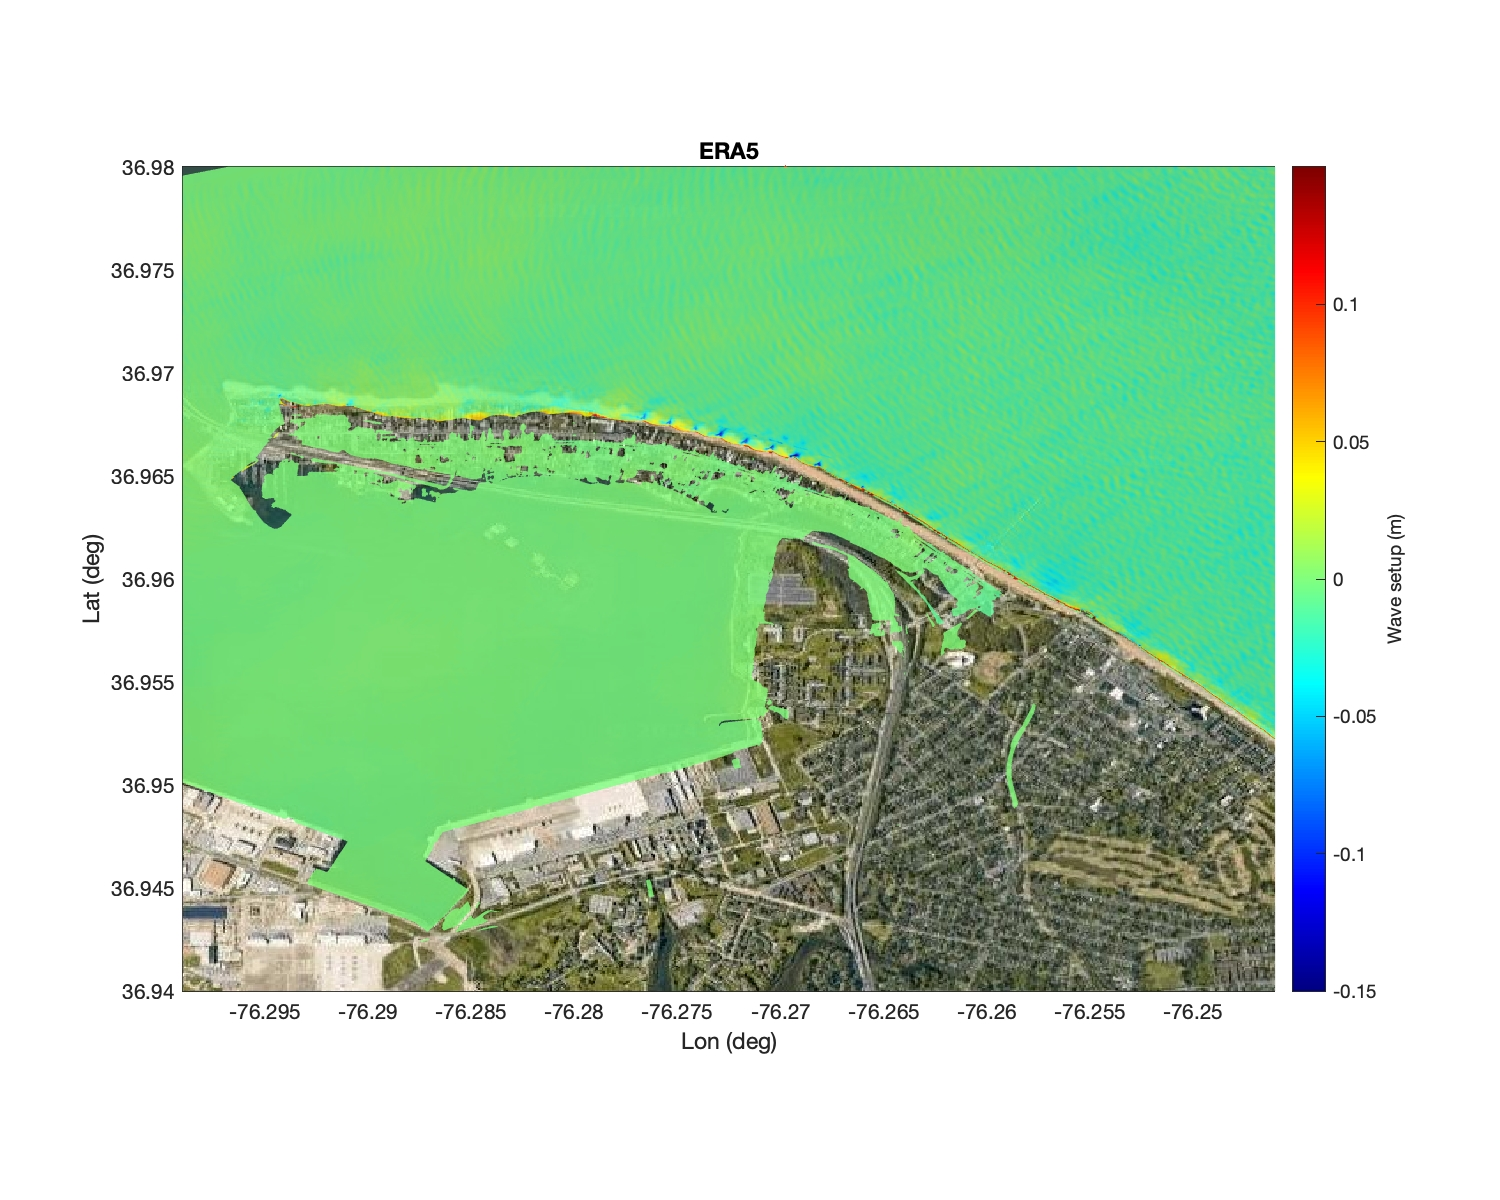
\includegraphics[width=\textwidth]{./figures/funwave_ERA5_setup.jpg}
\caption{FUNWAVE-TVD result of wave setup at the peak storm tide (27-Aug-2011 23:00) for scenarios ERA5.  }
\label{funwave_ERA5_setup}
\centering
\end{figure}

\begin{figure}
\centering
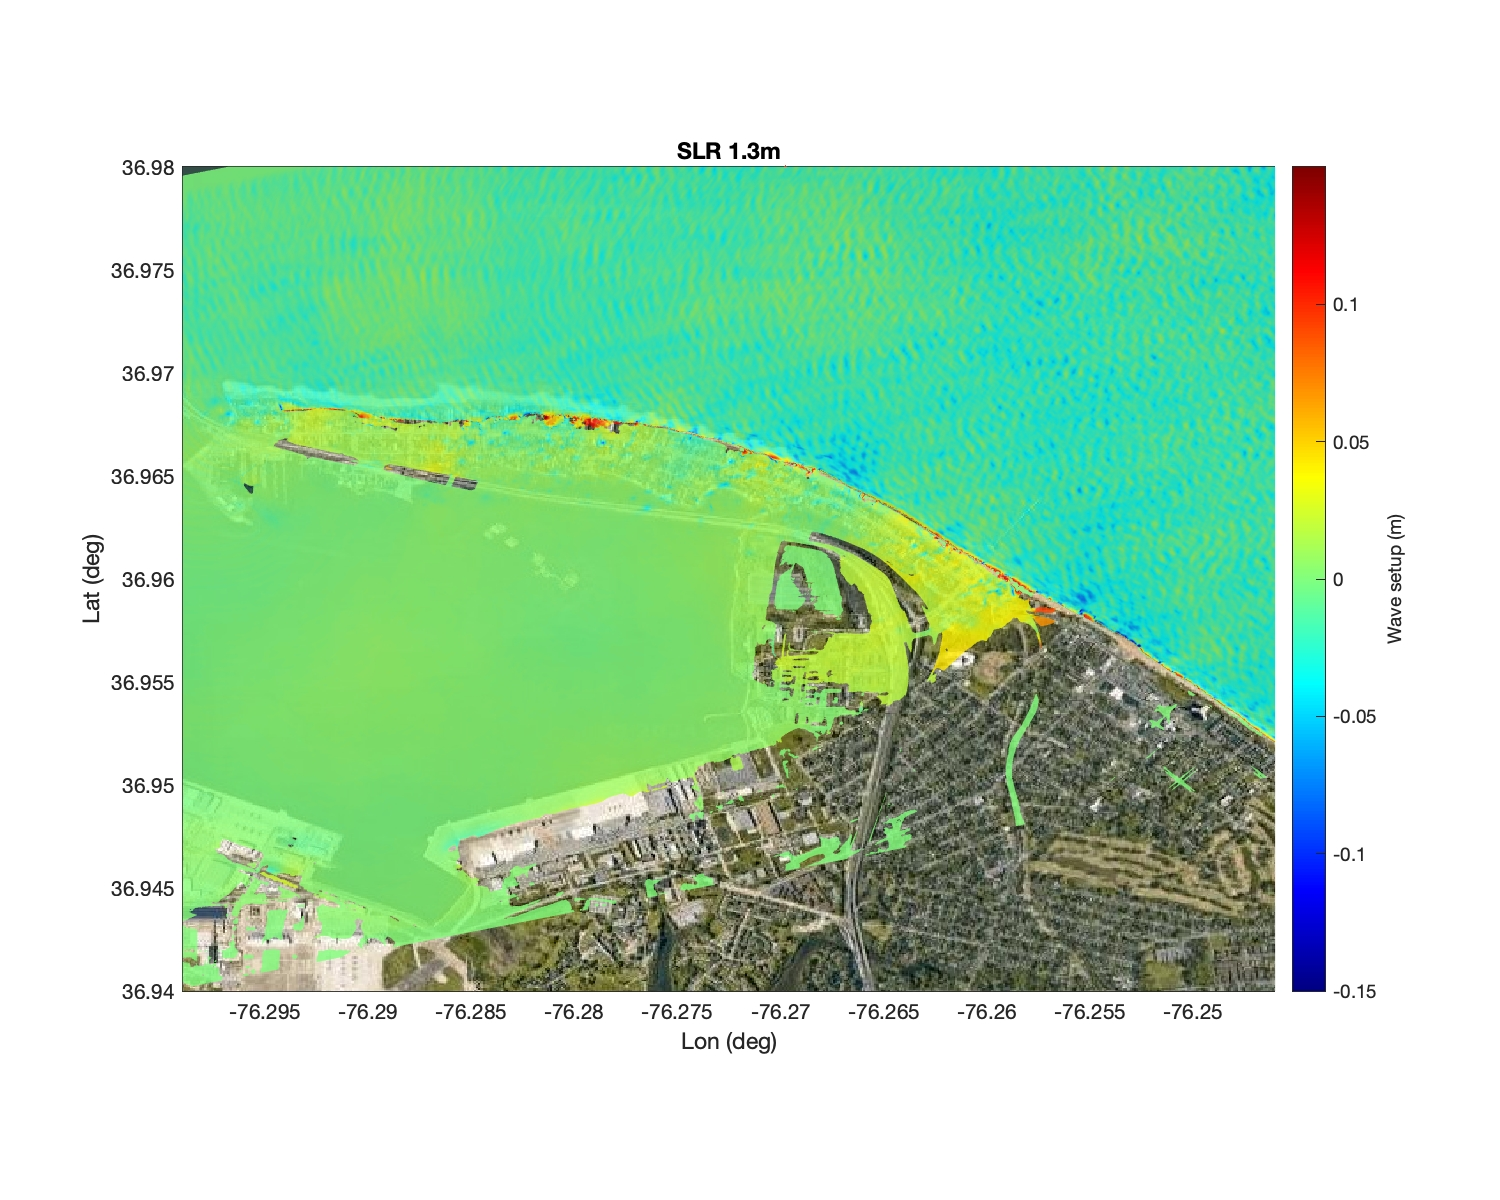
\includegraphics[width=\textwidth]{./figures/funwave_SLR_setup.jpg}
\caption{FUNWAVE-TVD result of wave setup at the peak storm tide (27-Aug-2011 23:00) for scenarios SLR 1.3 m. }
\label{funwave_SLR_setup}
\centering
\end{figure}

\begin{figure}
\centering
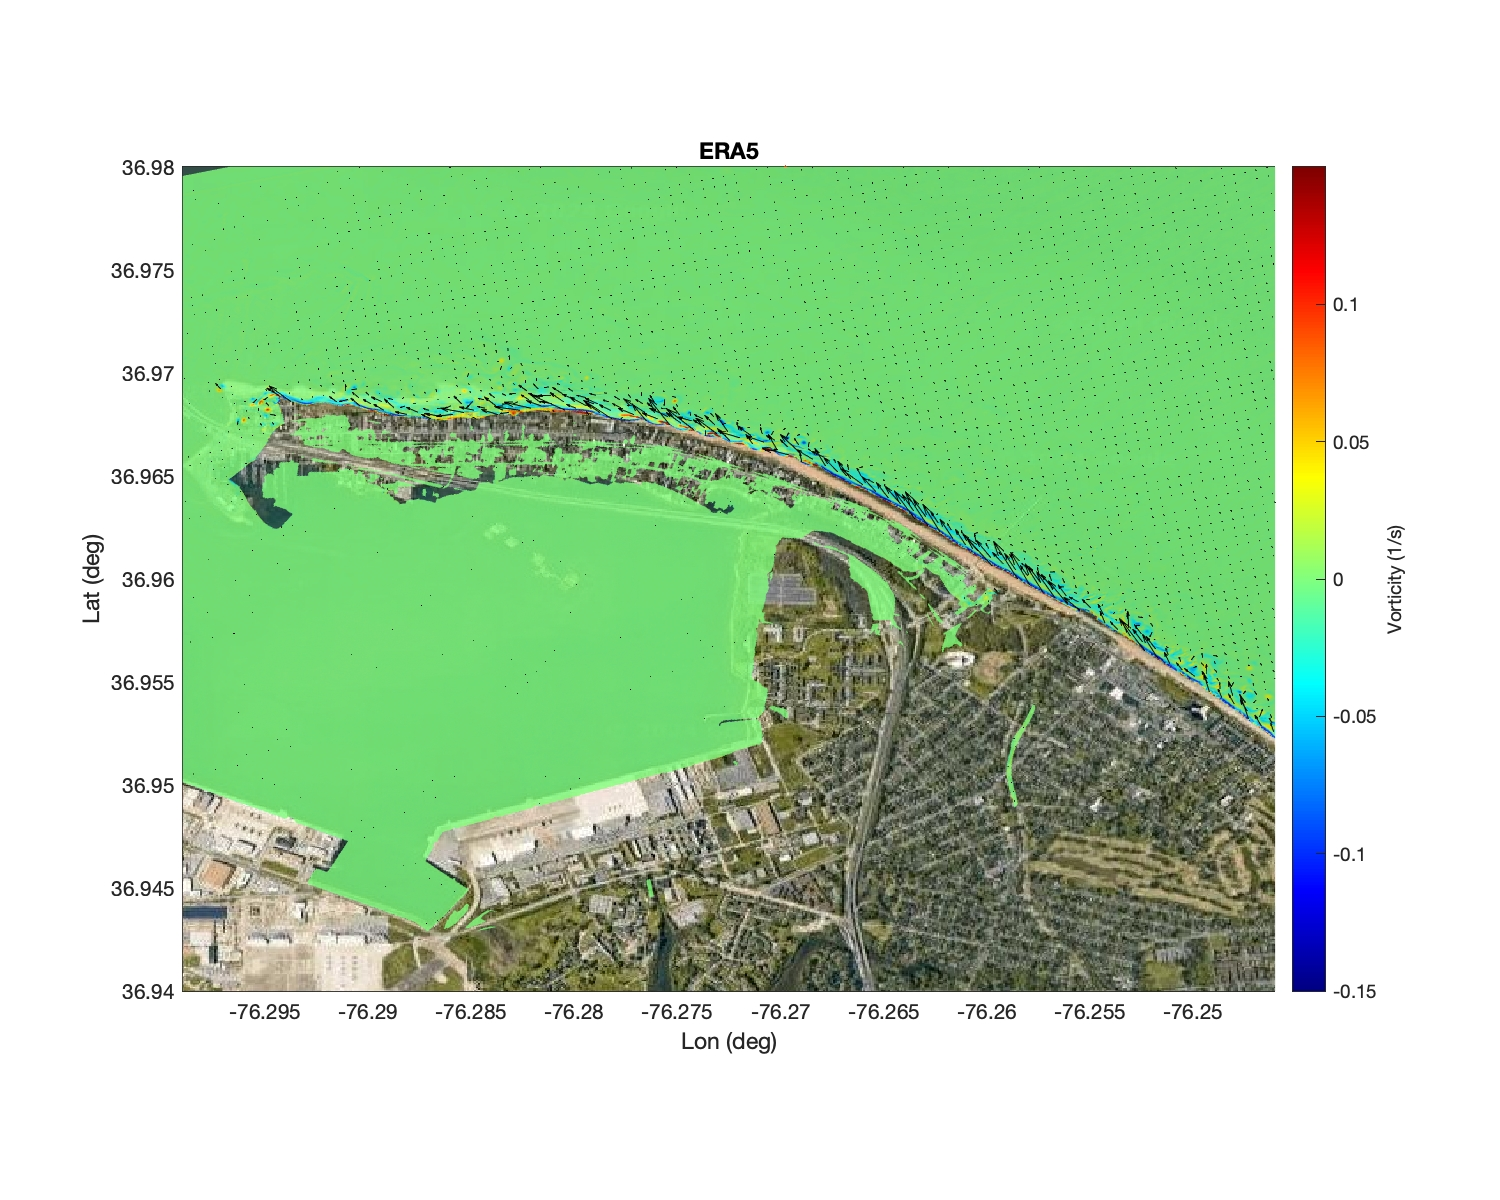
\includegraphics[width=\textwidth]{./figures/funwave_ERA5_vort.jpg}
\caption{FUNWAVE results of wave-induced current (vectors) and vertical vorticity (color) at the peak storm tide (27-Aug-2011 23:00) for scenarios ERA5. }
\label{funwave_ERA5_vort}
\centering
\end{figure}

\begin{figure}
\centering
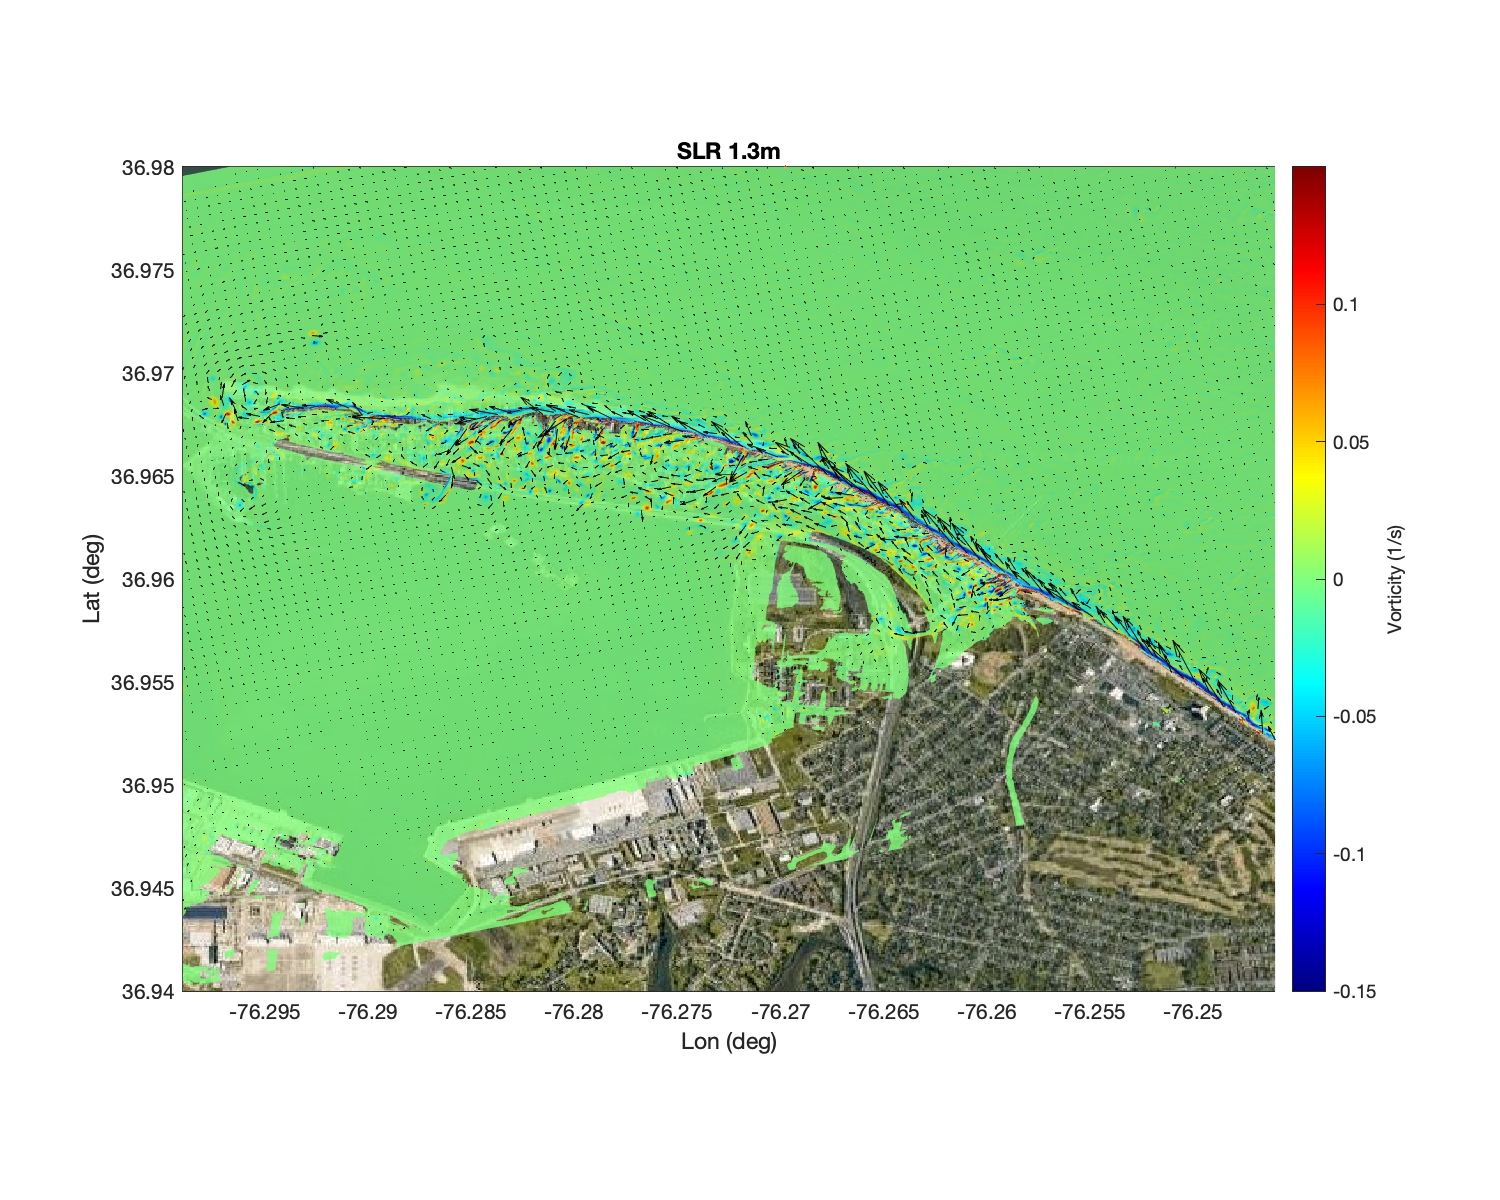
\includegraphics[width=\textwidth]{./figures/funwave_SLR_vort.jpg}
\caption{FUNWAVE results of wave-induced current (vectors) and vertical vorticity (color) at the peak storm tide (27-Aug-2011 23:00) for scenarios SLR 1.3 m.}
\label{funwave_SLR_vort}
\centering
\end{figure}

\begin{figure}
\centering
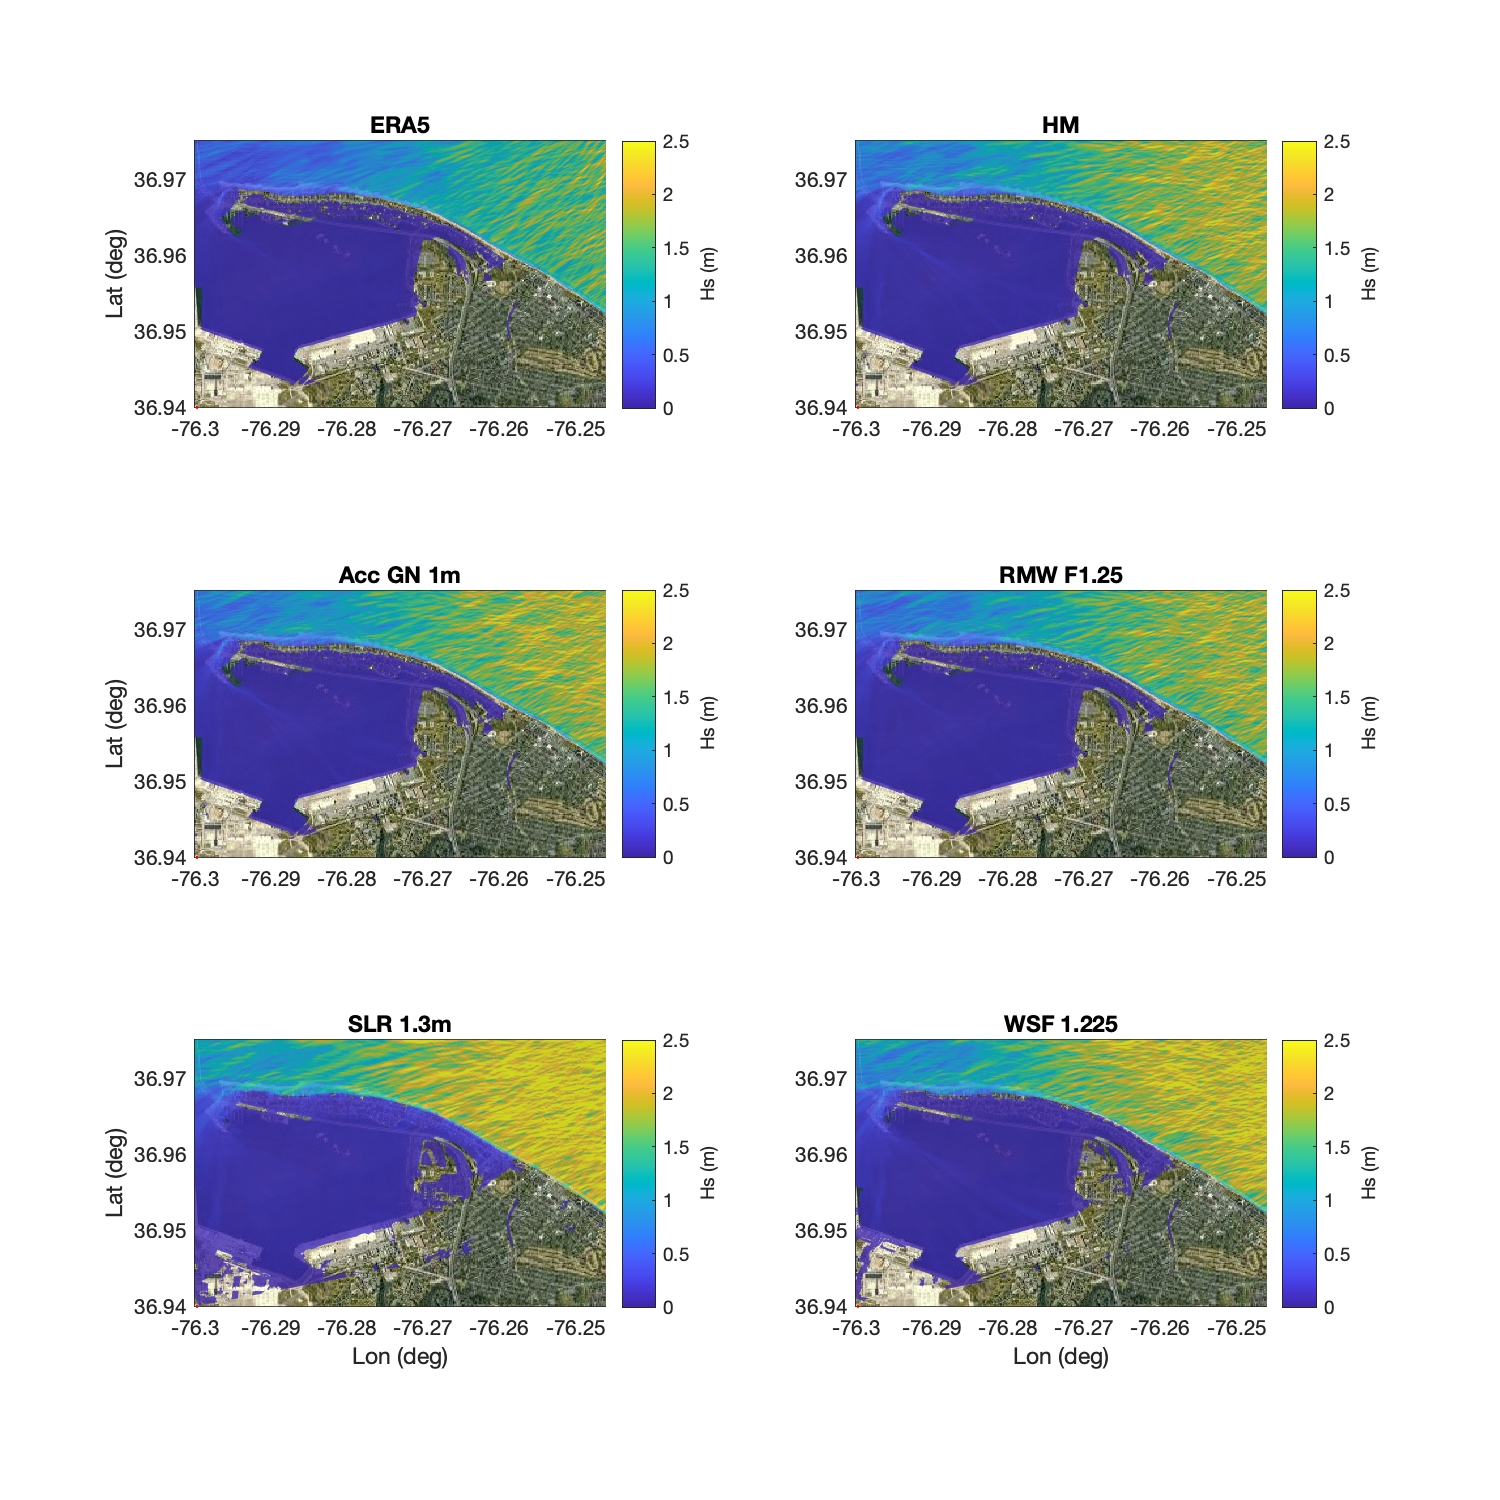
\includegraphics[width=\textwidth]{./figures/funwave_hs_6_cases.jpg}
\caption{FUNWAVE-TVD results of significant wave height  at the peak storm tide from the six selected scenarios. }
\label{funwave_6_cases_hs}
\centering
\end{figure}

\begin{figure}
\centering
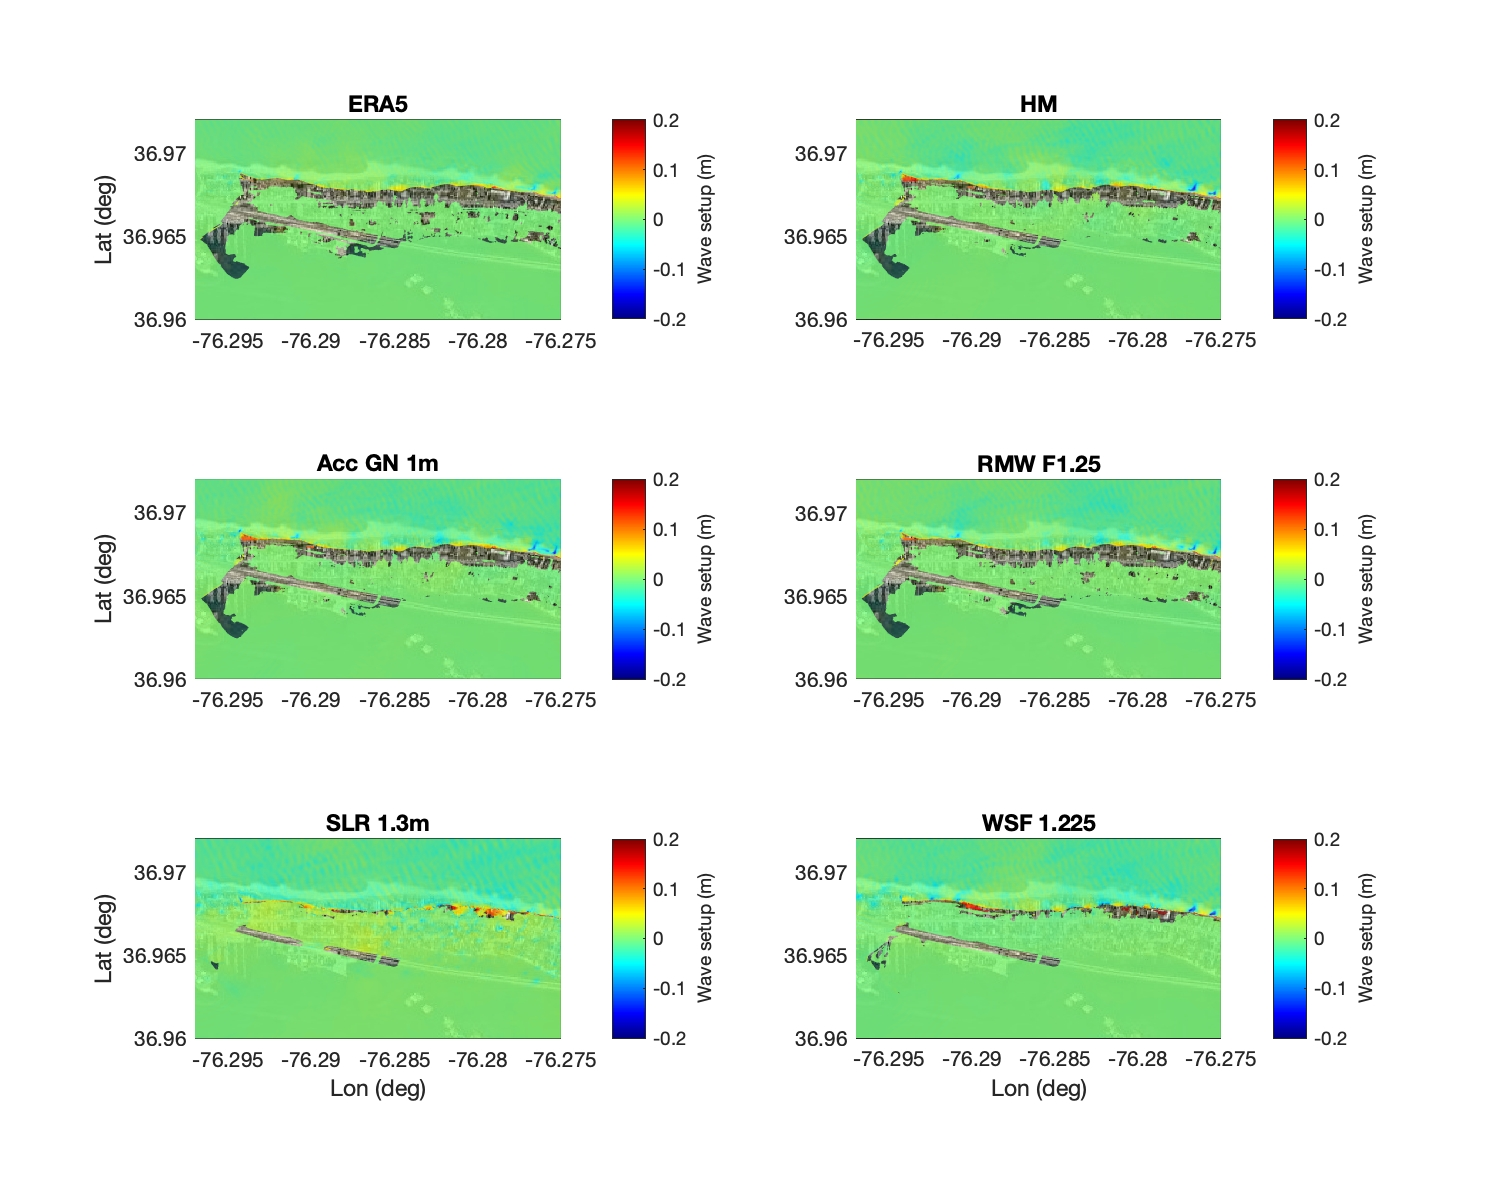
\includegraphics[width=\textwidth]{./figures/funwave_setup_6_cases.jpg}
\caption{FUNWAVE-TVD results of wave setup  at the peak storm tide from the six selected scenarios. }
\label{funwave_6_cases_setup}
\centering
\end{figure}

\begin{figure}
\centering
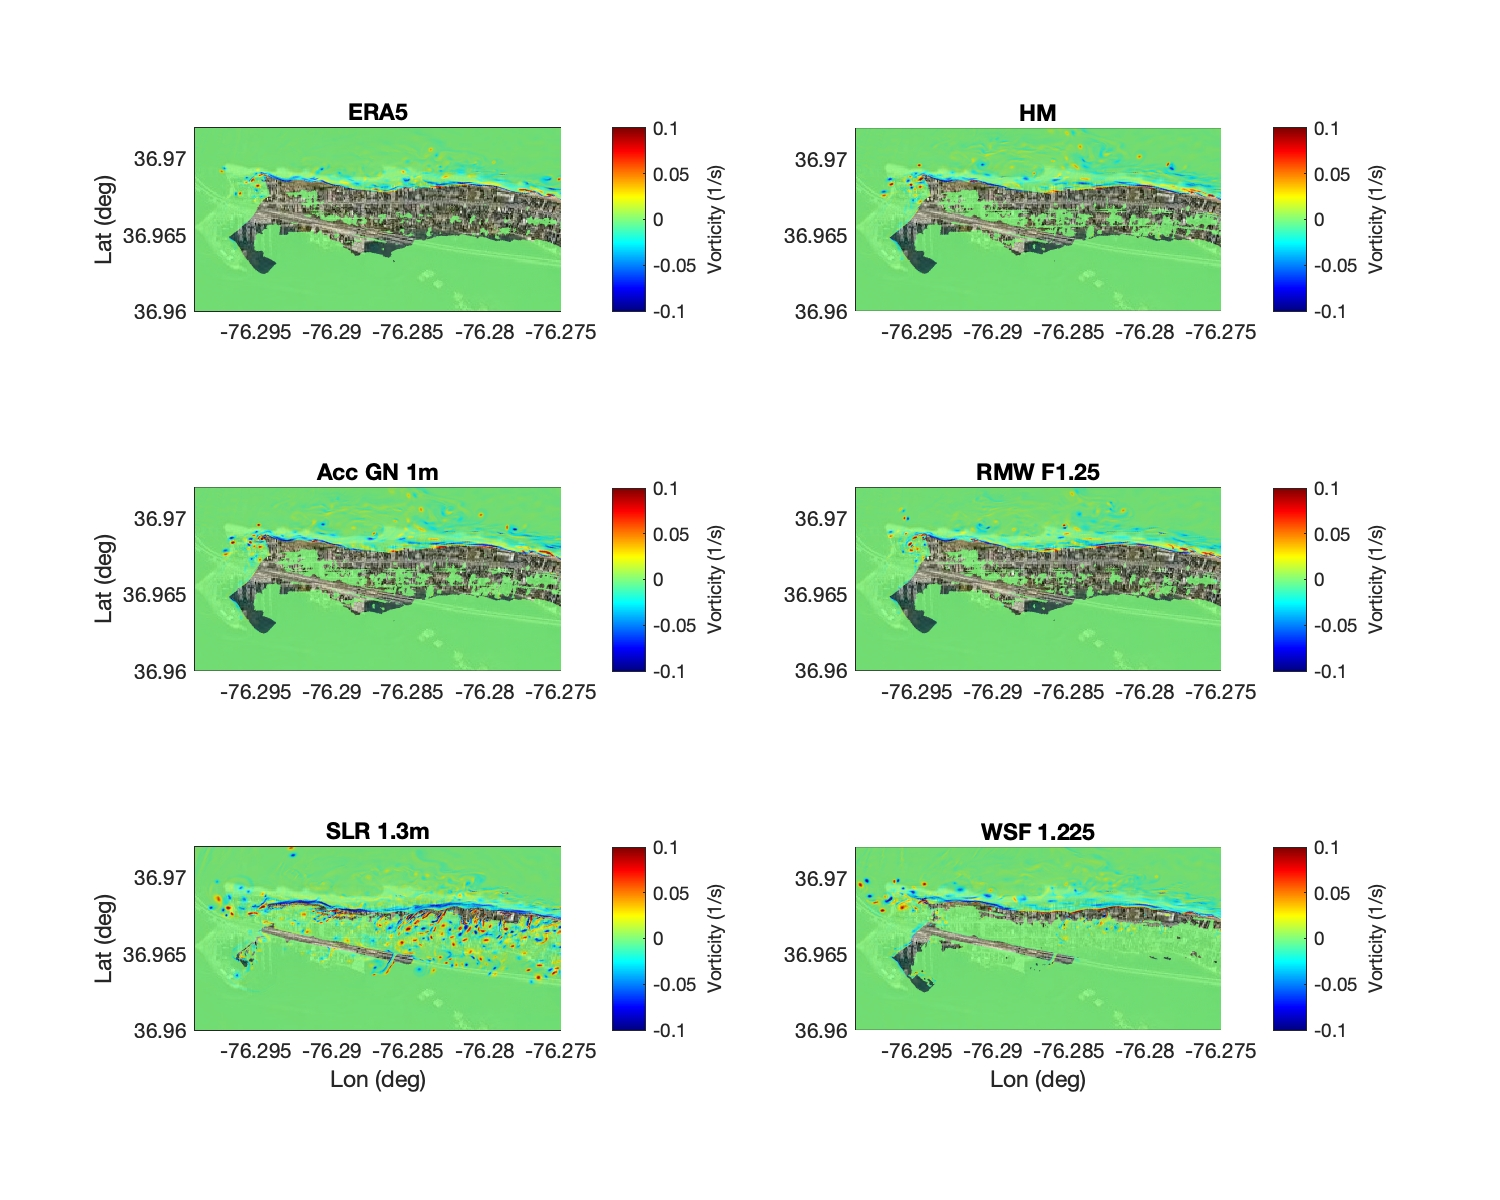
\includegraphics[width=\textwidth]{./figures/funwave_vort_6_cases.jpg}
\caption{FUNWAVE-TVD results of wave-induced vorticity  at the peak storm tide from the six selected scenarios.}
\label{funwave_6_cases_setup}
\centering
\end{figure}

\bibliographystyle{elsarticle-harv}

\biboptions{authoryear}
%\bibliographystyle{elsarticle-num}
\bibliography{bbh}
\end{document}